\documentclass[aspectratio=169,10pt]{imta}

\usepackage{config}

\title{RADAR: Model Quality Assessment for Reputation-aware Collaborative Federated Learning}

\subtitle{}

\author{
  \textbf{Léo Lavaur}\inst{1,3} \and
  \textbf{Pierre-Marie Lechevalier}\inst{1,4} \and
  Y. Busnel\inst{2,3} \and
  R. Ludinard\inst{1,3} \and
  G. Texier\inst{1,4} \and
  M.-O. Pahl\inst{1,3}
}

\institute{
  \inst{1}IMT Atlantique \quad
  \inst{2}IMT Nord Europe \quad
  \inst{3}SOTERN (IRISA) \quad
  \inst{4}ADOPNET (IRISA)

  \vfill\footnotesize
  {leo.lavaur@imt-atlantique.fr}\\
  {pierre-marie.lechevalier@imt-atlantique.fr}
  
}

\date{43\textsuperscript{rd} International Symposium on Reliable Distributed Systems (Sep.--Oct. 2024)}

\setlength{\logosize}{1.5cm}
\titlegraphic{%
  \raisebox{-0.5\height}{
\includegraphics[height=\logosize,keepaspectratio]{logos/imt-atlantique.pdf}}%
  \raisebox{-0.5\height}{
\includegraphics[height=.75\logosize,keepaspectratio]{logos/cybercniGB.pdf}}%
  \hspace{10pt}%
  \raisebox{-0.5\height}{
\includegraphics[height=.75\logosize,keepaspectratio]{logos/b5g.png}}%
}

\subject{Federated Learning; Intrusion Detection; Byzantine; Cross-evaluation; Similarity; Clustering; Reputation Systems; Trust; Heterogeneity}

%%%%%%%%%%%%%%%%%%%%%%%%%%%%%%%%%%%%%%%%%%%%%%%%
%%%%            DOCUMENT CONTENT            %%%%
%%%%%%%%%%%%%%%%%%%%%%%%%%%%%%%%%%%%%%%%%%%%%%%%

\begin{document}

\maketitle
% Introduction
% -----------------------------
%\section*{Introduction}

% \begin{frame}{Intrusion Detection Use Case}

%     \begin{block}{Intrusion Detection System (IDS)}
%         IDSs monitor the behavior of a system to detect malicious activities.
%     \end{block}
%     \hfill
%     \pause
%     \begin{block}{Collaborative IDSs (CIDSs)}
%         CIDSs share information between \alert<3>{distributed parties} (whether they are automated probes, collection points, or legal entities) to improve the characterization of malicious activities, thus facilitating their detection.
%     \end{block}

% \end{frame}



% \begin{frame}{Scaling Intrusion Detection}
\begin{frame}{Federated Learning Primer}

  \begin{columns}
    \begin{column}{0.4\textwidth}
      \textbf{Federated Learning (FL)}
      \small
      \begin{itemize}[<+->]
        \item Distributed ML paradigm (Google, 2017)~\autocite{mcmahan_Communicationefficientlearningdeep_2017}.
        \item Distributed clients  train a common model without sharing training data.
        \item \alert{Privacy-preserving}: high level of abstraction for the shared models, preventing data leakage.
      \end{itemize}
    \end{column}
    
    \begin{column}{0.6\textwidth}
      \begin{figure}
        \centering
        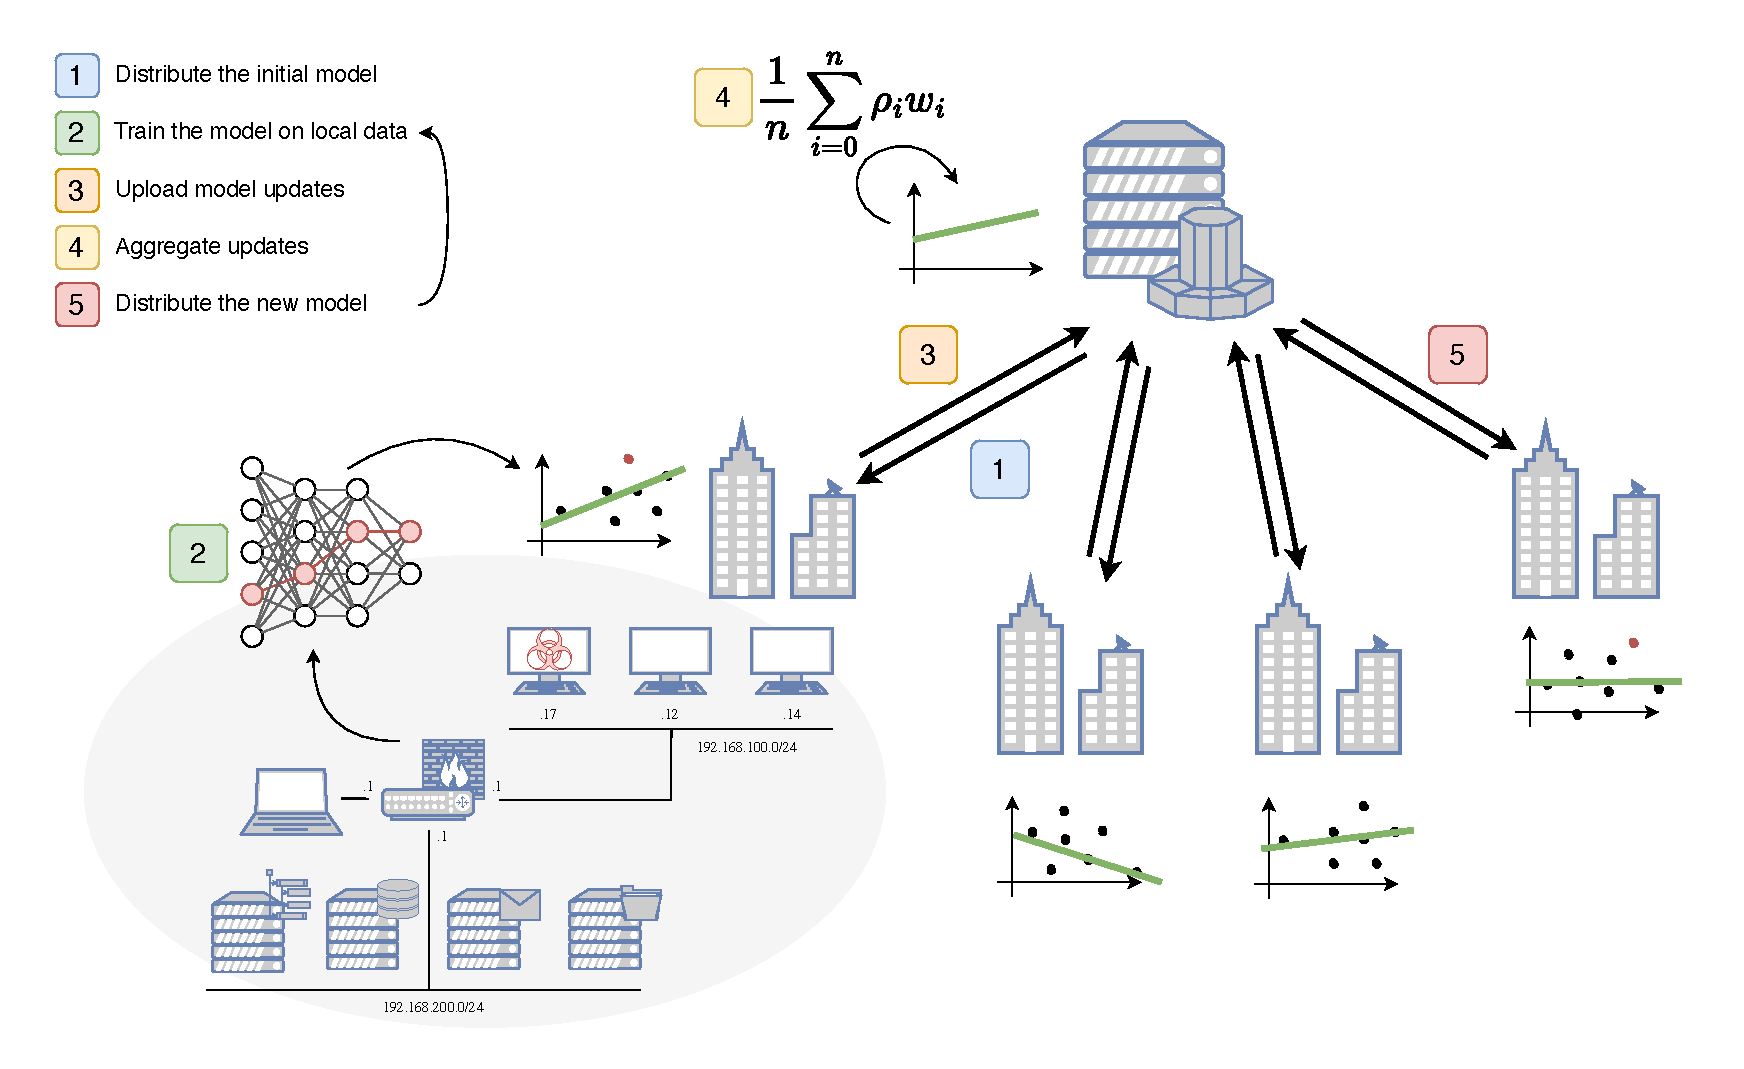
\includegraphics[width=1.1\linewidth,right]{figures/intro/fl.drawio.pdf}
      \end{figure}
    \end{column}
  \end{columns}

  \fcitefootnote{mcmahan_Communicationefficientlearningdeep_2017}
\end{frame}

\begin{frame}{Case Study -- Collaborative IDS}

  \begin{columns}
    \begin{column}{0.4\textwidth}
      \textbf{Collaborative Intrusion Detection between Distributed Organizations}
  \begin{itemize}[<+->]
    \item One NIDS and one monitored network per organization.
    \item Objective: improve their local detection performance.
    \item Means:
    \begin{itemize}
        \item expert knowledge (\ie, datasets),
        \item computing resources (\ie, model training).
    \end{itemize}
  \end{itemize}
    \end{column}
    
    \begin{column}{0.6\textwidth}
      \begin{figure}
        \centering
        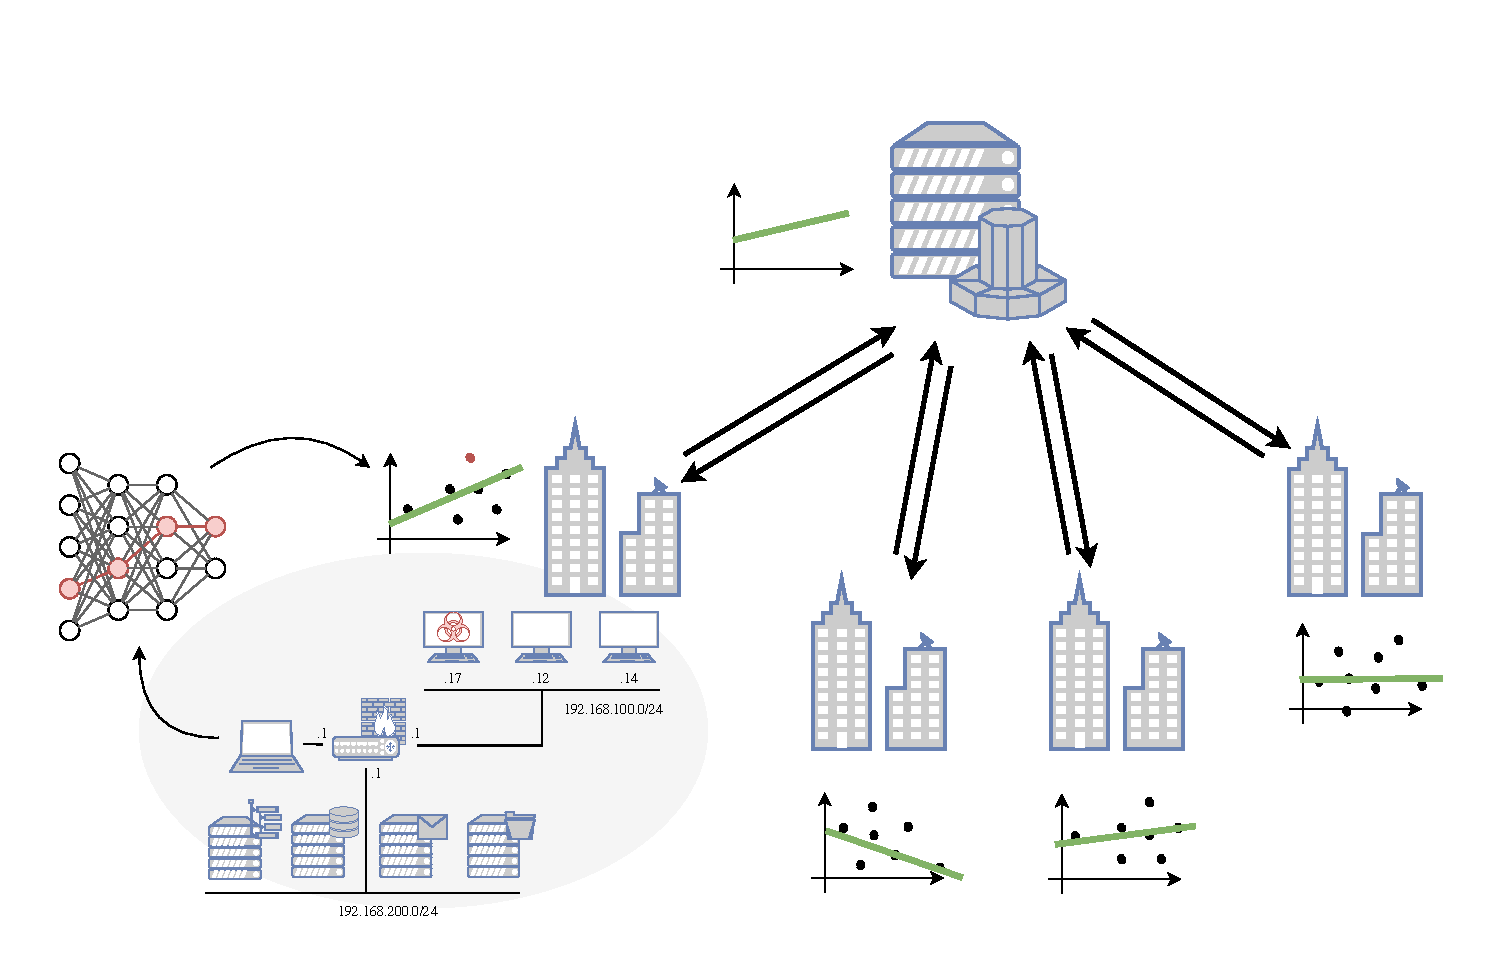
\includegraphics[width=1.1\linewidth,right]{figures/intro/cids.drawio.pdf}
      \end{figure}
    \end{column}
  \end{columns}
\end{frame}



\begin{frame}{Case Study -- Byzantine Contributions}
\begin{columns}
    \begin{column}{0.4\textwidth}
      \begin{itemize}
        \item No guarantees on the quality of the contributions.
        \item Intentional, due to poor data quality, or due to data distribution mismatches.
      \end{itemize}
      
      $\rightarrow$ \textbf{Byzantine contributions}
    \end{column}
    
    \begin{column}{0.6\textwidth}
      \begin{figure}
        \centering
        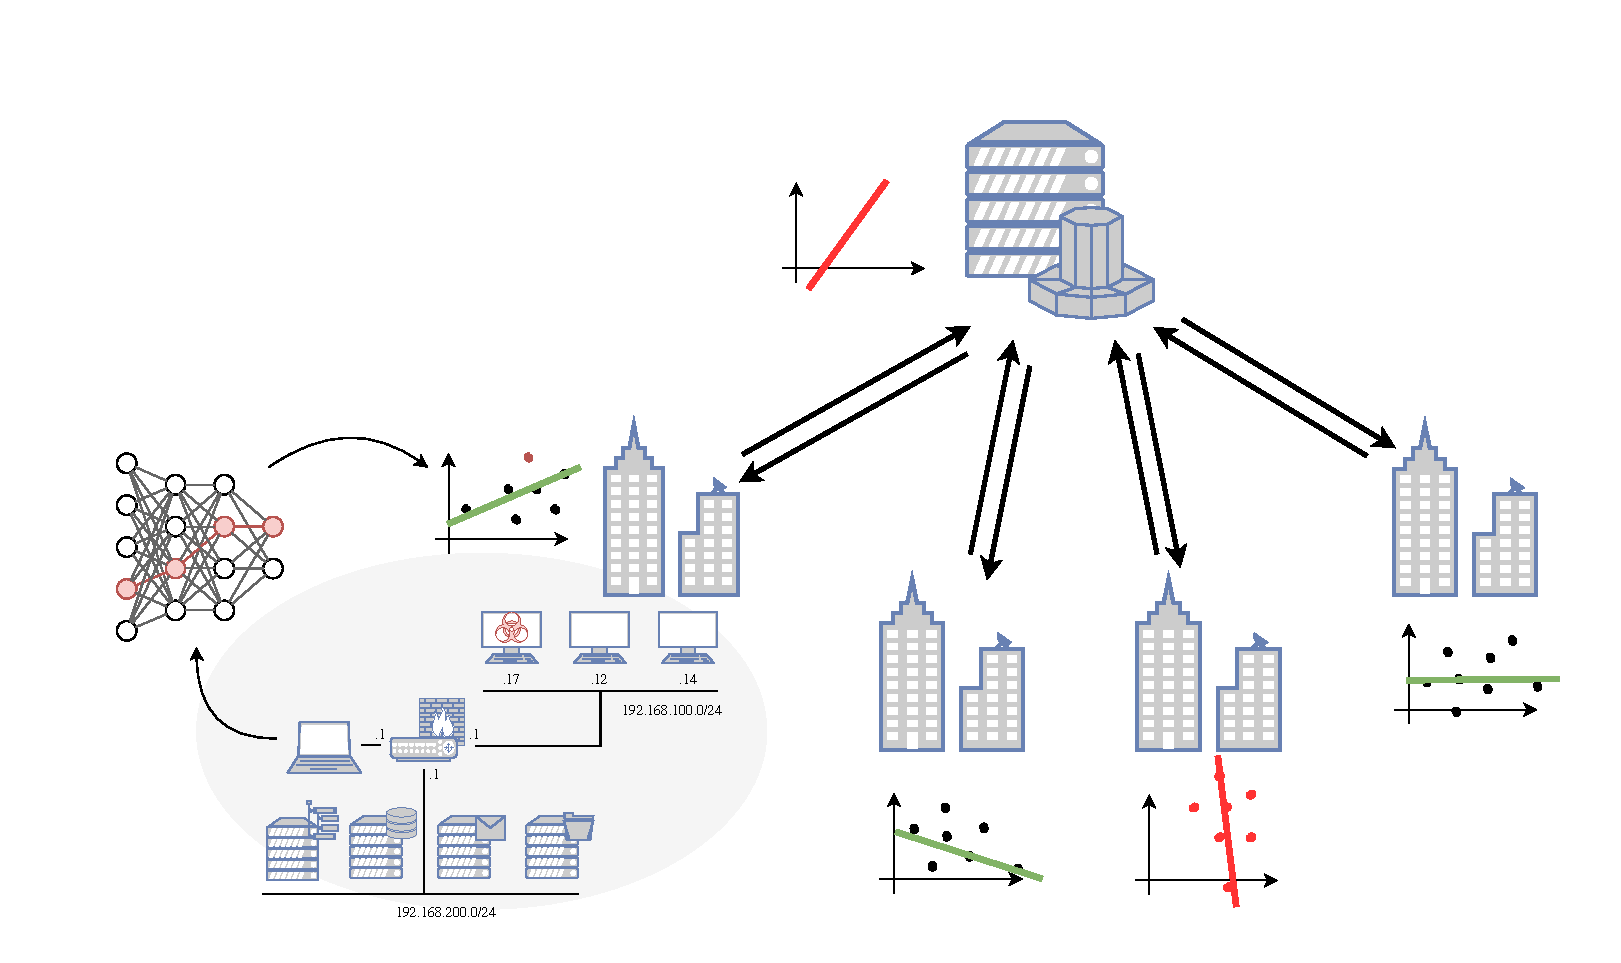
\includegraphics[width=1.1\linewidth,right]{figures/intro/poisoning.drawio.pdf}
      \end{figure}
    \end{column}
  \end{columns}
\end{frame}

\begin{frame}{Case Study -- Generalization}
  \textbf{A cross-silo use case}~\cite{kairouz_AdvancesOpenProblems_2021}:
  \begin{itemize}
    \item few clients (\ie, 10--100);
    \item consequent amount of data, high heterogeneity;
    \item high availability, significant computing resources;
    \item untrusted participants, honest server.
  \end{itemize}
\end{frame}

\begin{frame}{Heterogeneity Headaches}
  
  \begin{columns}
    \begin{column}{.5\textwidth}
      \includegraphics<1>[width=\linewidth]{figures/intro/heterogeneity/introducing_heterogeneity_aggregated.pdf}
      \includegraphics<2>[width=\linewidth]{figures/intro/heterogeneity/introducing_poisoning.pdf}

    \end{column}

    \begin{column}{.5\textwidth}

      \textcolor<2->{lightgray}{%
      \textbf{Challenge I}: \textit{Too much heterogeneity leads to poor performance\dots}
      }
      \only<1>{%
        \begin{itemize} \small
          \item How to handle different feature sets, data distributions?
          \item How to consider models that are dissimilar yet "contain" relevant knowledge?
        \end{itemize}
      }
      \vspace{1ex}


      \textcolor<1>{lightgray}{%
      \textbf{Challenge II}: \textit{Difficult to identify malicious contributions when models are different\dots}
      }
      
      \only<2>{%
        \begin{itemize} \small
          \item Are model "dissimilar" because they are different, or because they are malicious/poisoned?
        \end{itemize}
      }
      \vspace{1ex}
      
    \end{column}
  \end{columns}  
\end{frame}

\begin{frame}{Problem Statement}
% Reformuler 
  \begin{block}{Quality Assessment in Heterogeneous Settings}
    In a context where multiple participants own datasets of \alert{unknown similarity}, each participant contributes a local model update at each round. 
    
    How can one assess the \alert{contribution quality} of each participant’s local models without making assumptions on the \alert{participant data distribution} ?
  \end{block}
  % \begin{block}{Quality Assessment in Heterogeneous Settings}
  %   For $n$ participants $p_i$ and their local datasets $d_i$ of unknown similarity, each participant uploads a model update $w_i^r$ at each round $r$. Given $P = \{ p_1, p_2, \dots, p_n \} $ and $W = \{ w_1^r, w_2^r, \dots, w_n^r \} $, how can one assess the quality of each participant’s contribution without making assumptions on the data distribution across the datasets $d_i$?
  % \end{block}
\end{frame}

\begin{frame}{Existing Solutions}

  \begin{columns}[T]
    
    \begin{column}{.33\textwidth}
      \small\centering
      \textbf{Server-side evaluation}~\autocite{zhou_DifferentiallyPrivateFederated_2022}

      \begin{figure}
        \centering
        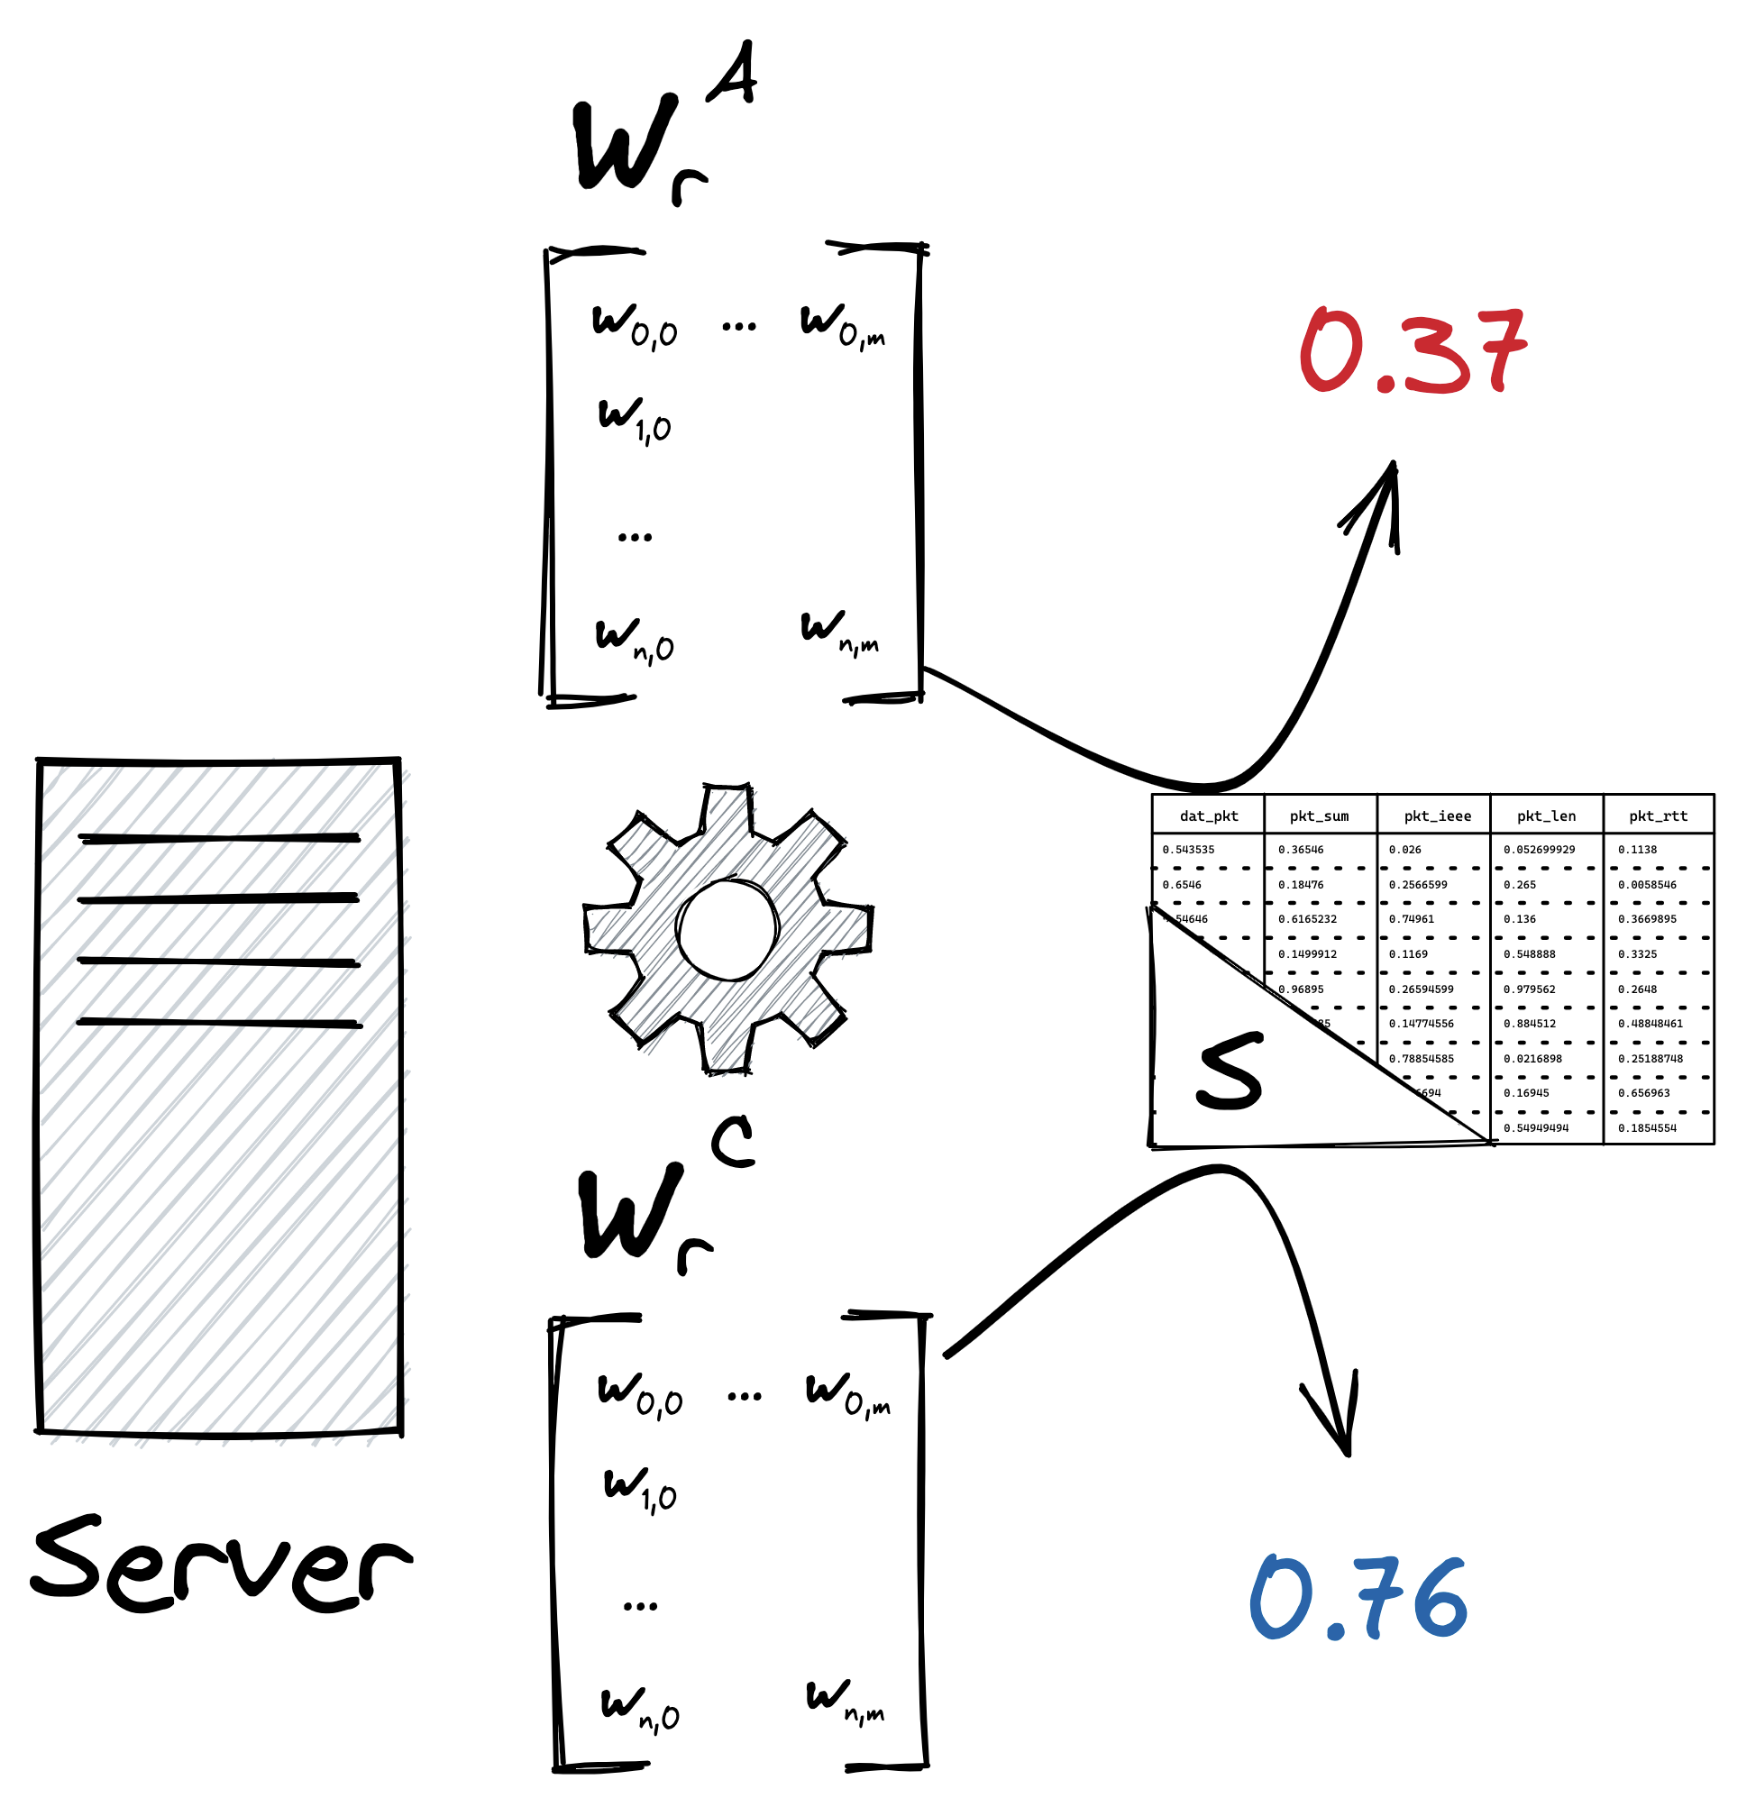
\includegraphics[height=.36\textheight]{figures/radar/server-side-eval}
      \end{figure}

      \begin{itemize}\smaller
        \item Only applicable in IID settings.
        % \item Single source of truth.
      \end{itemize}
    \end{column}

    \onslide<2->{%
      \begin{column}{.33\textwidth}
        \small\centering
        \textbf{Server-side comparison}~\autocite{briggs_Federatedlearninghierarchical_2020}

        \begin{figure}
          \centering
          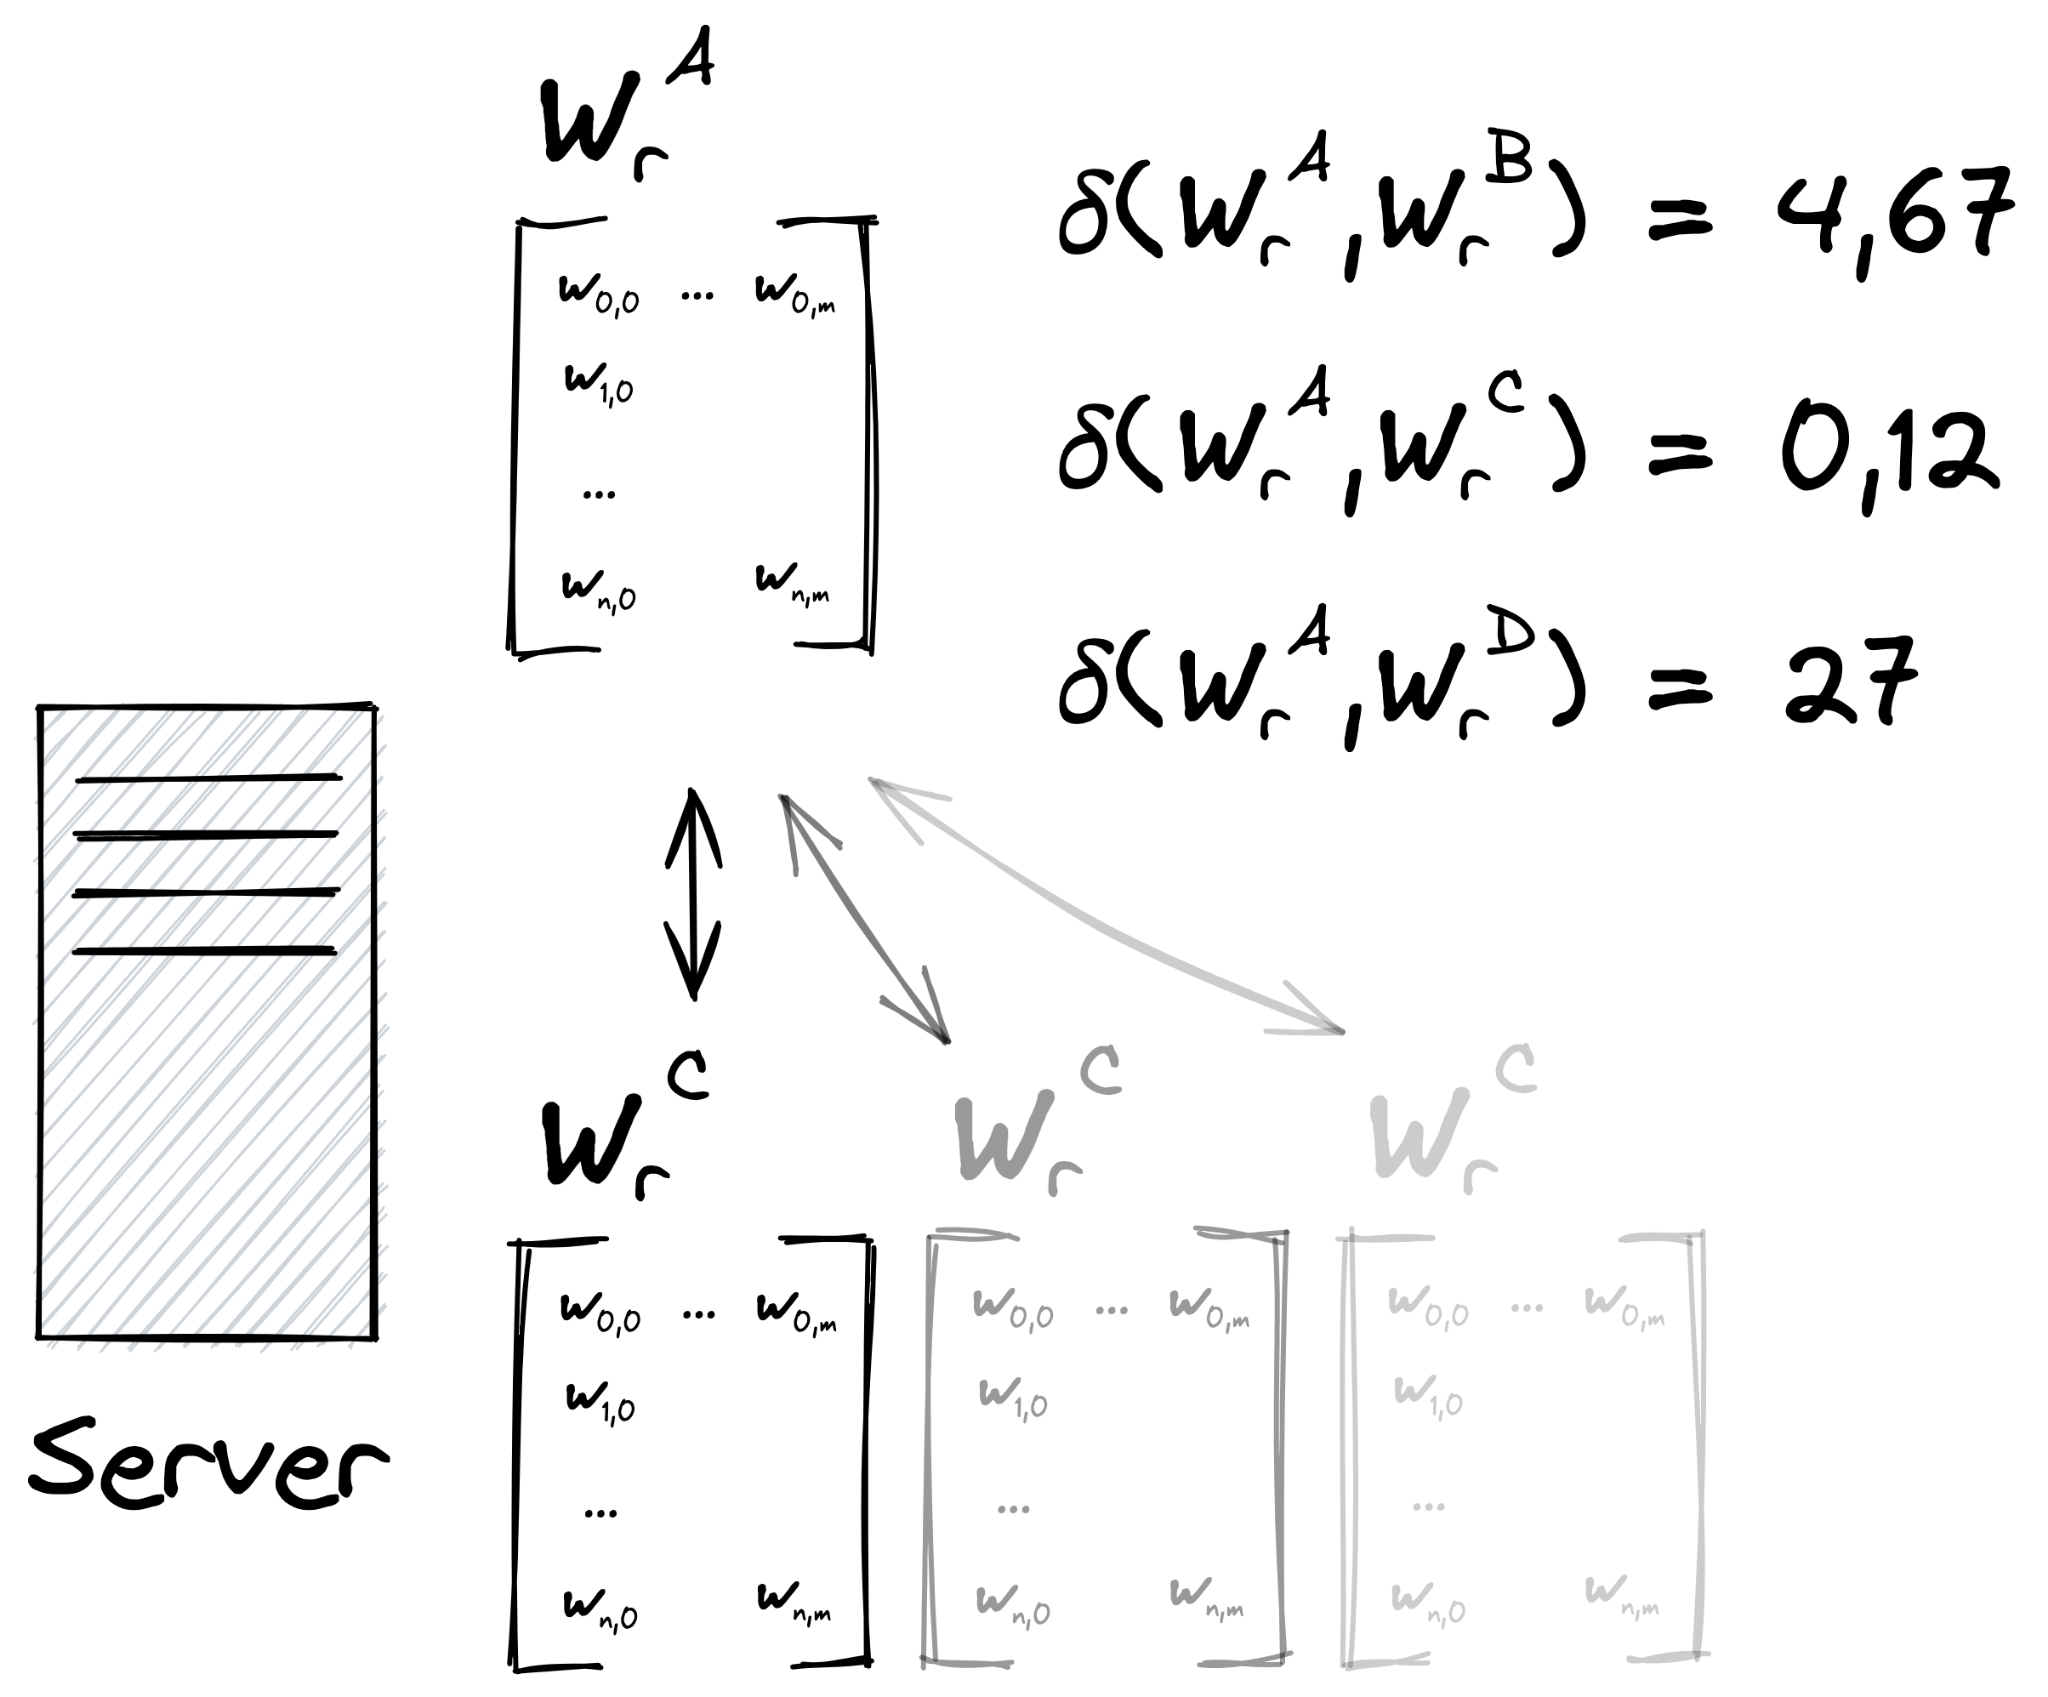
\includegraphics[height=.36\textheight]{figures/radar/server-side-comp}
        \end{figure}

        \begin{itemize}\smaller
          \item Less related to client data.
          % \item More appropriate for high-dimensional data.
        \end{itemize}
      \end{column}%
    }

    \onslide<3->{%
      \begin{column}{.33\textwidth}
        \small\centering
        \textbf{Client-side evaluation}~\autocite{zhao_ShieldingCollaborativeLearning_2020}

        \begin{figure}
          \centering
          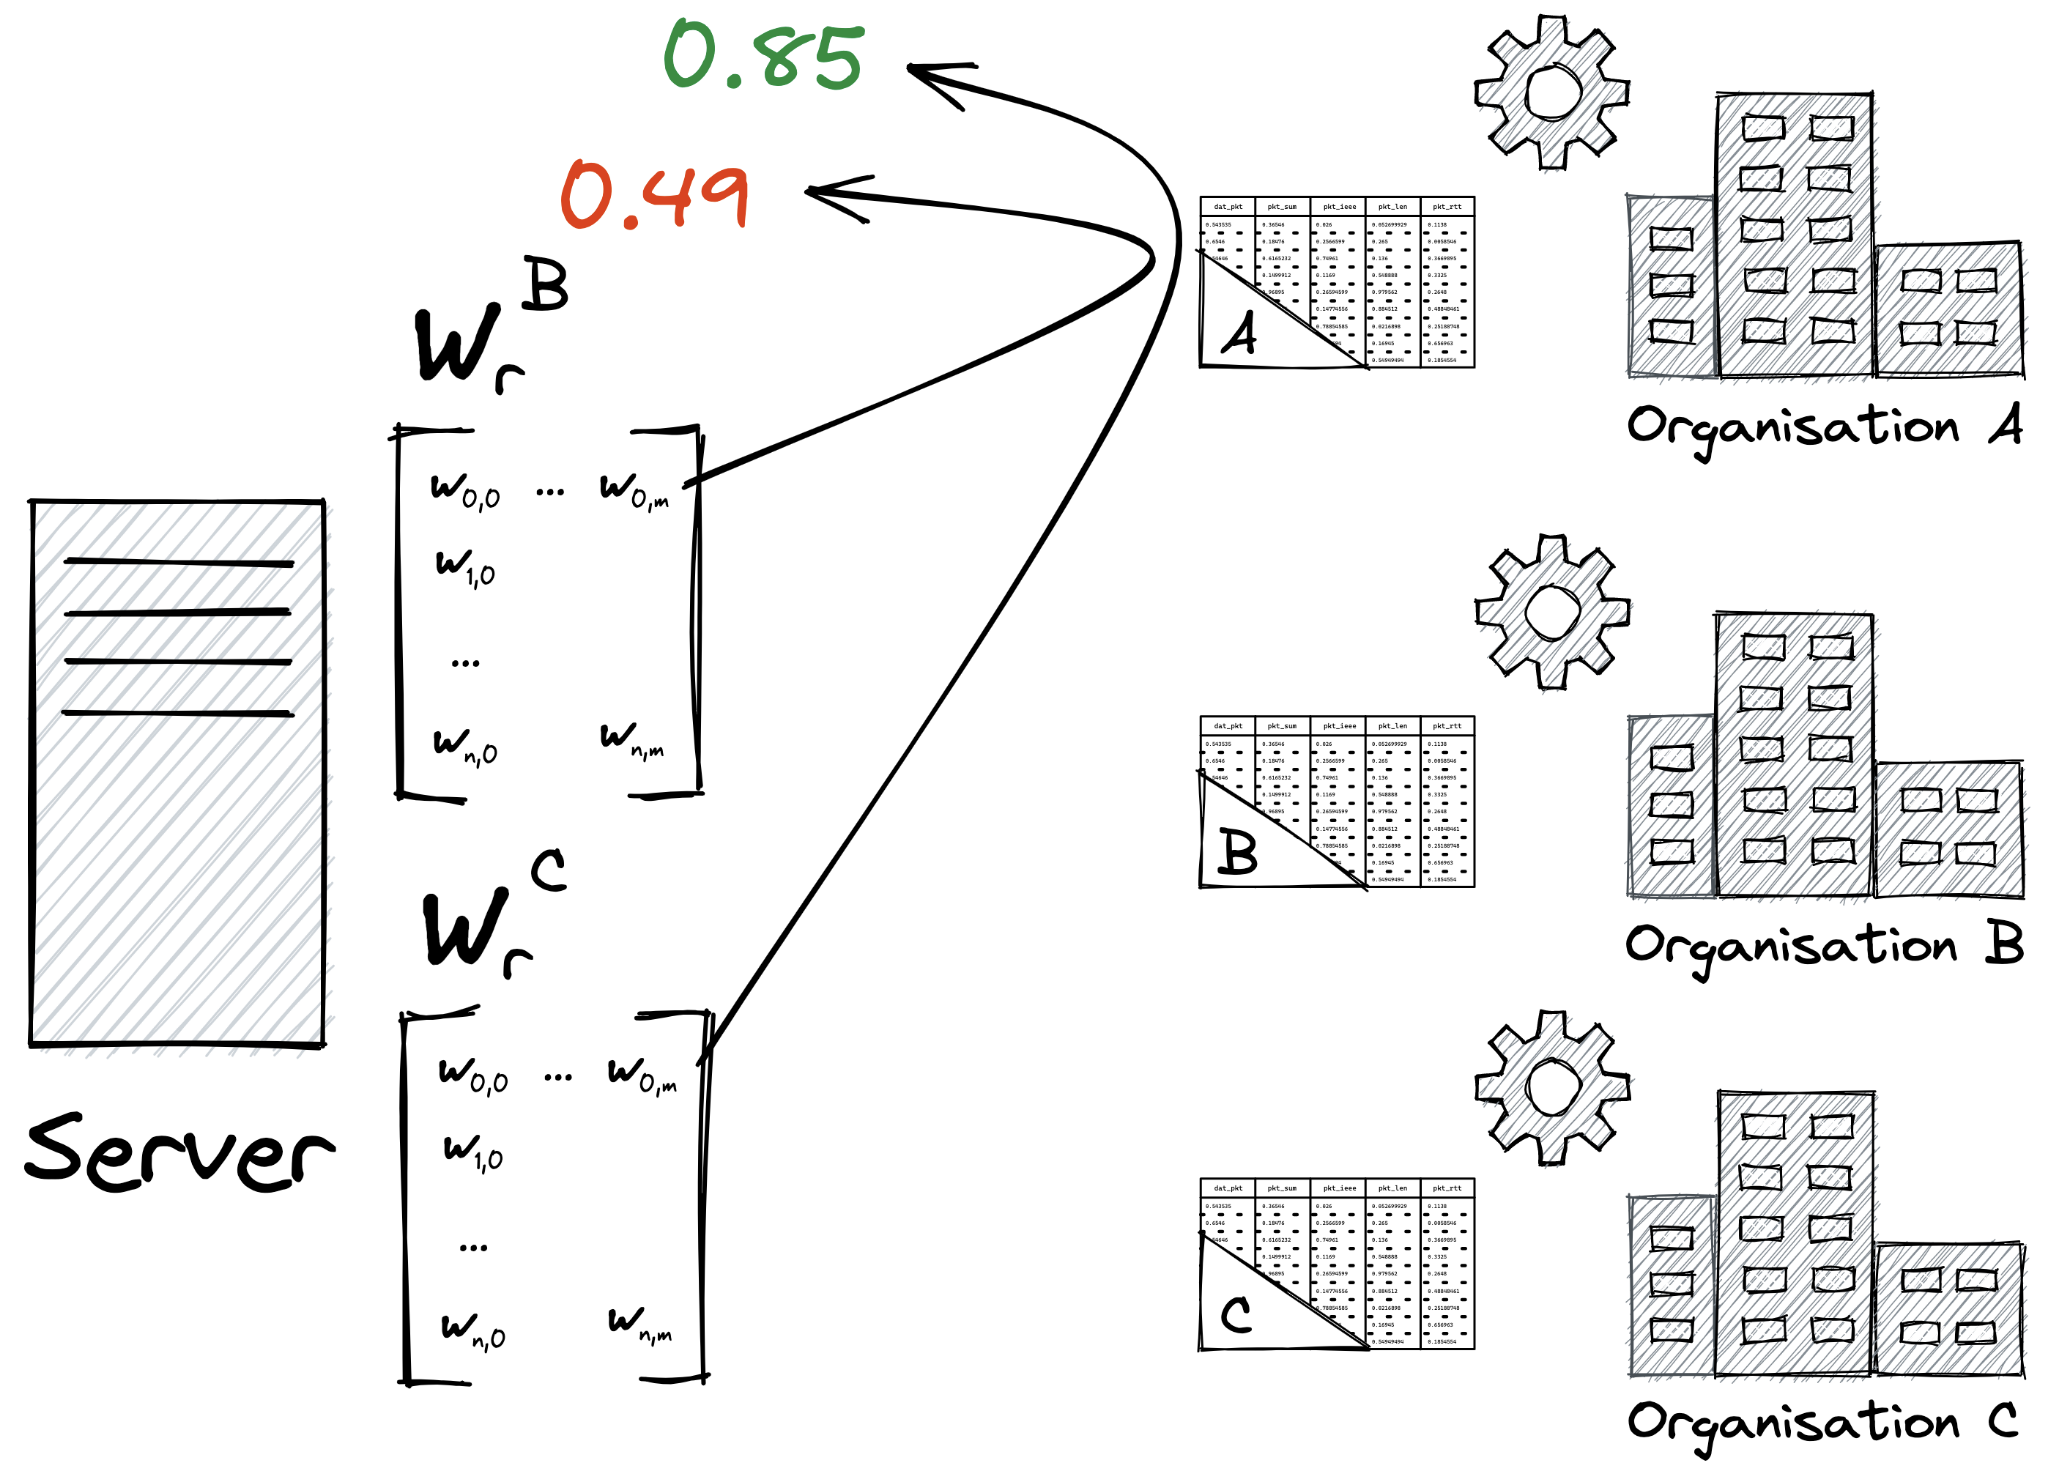
\includegraphics[height=.36\textheight]{figures/radar/client-side-eval}
        \end{figure}

        \begin{itemize}\smaller
          \item High cost in cross-device.
          % \item More susceptible to badmouthing.
        \end{itemize}
      \end{column}%
    }

  \end{columns}

  \vspace{3ex}
  
  \fcitefootnote{zhou_DifferentiallyPrivateFederated_2022}
  \only<1>{\blankfootnote{}} % To keep the same height for the footnotes.
  \only<2->{\fcitefootnote{briggs_Federatedlearninghierarchical_2020}}
  \only<3->{\fcitefootnote{zhao_ShieldingCollaborativeLearning_2020}}

\end{frame}

\begin{frame}{Architecture}
  \centering
    \begin{figure}
        \centering
        \includegraphics<1>[width=.95\linewidth,left]{figures/radar.pdf}%
        \caption*{\texttt{RADAR} architecture. } % remove Figure:
        \label{fig:radar}
    \end{figure}  
         
    % \tableofcontents%[hideallsubsections,]
\end{frame}



% Architecture
% -----------------------------
%\section{Architecture}
\subsection{Assessing Contribution Quality}
\begin{frame}
    \tikz[overlay, remember picture,
      shift=(current page.south west),
      x=(current page.south east),
      y=(current page.north west)
    ]{
        % Show the optional help grid lines 
        %\draw[step=.1, opacity=0.3, thick, red] (0,0) grid (1,1);
      
        \node[anchor=south east] at (1,0) {
            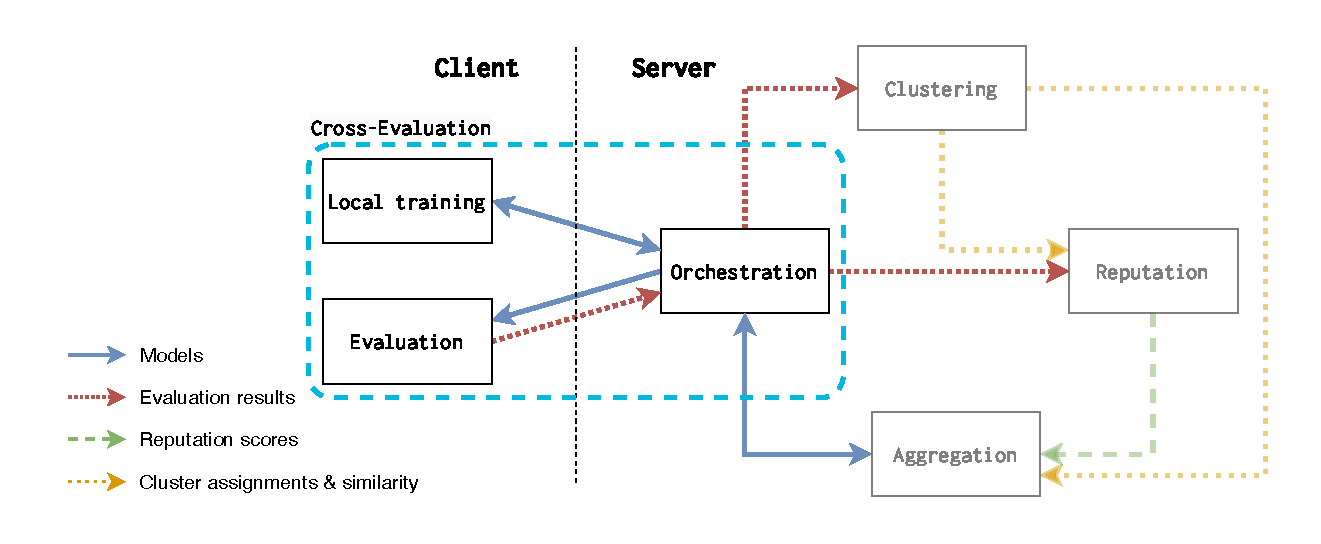
\includegraphics[width=\textwidth]{figures/radar-xeval.pdf}
        };
        
        \node[align=left, anchor=north west] at (.05,.91) {\begin{minipage}{.7\textwidth}\subsectionpage\end{minipage}};
    }
\end{frame}

\begin{frame}{Assessing Quality with Cross-Evaluation}

  \begin{columns}
    \begin{column}{.45\textwidth}
      \begin{figure}
        \centering
        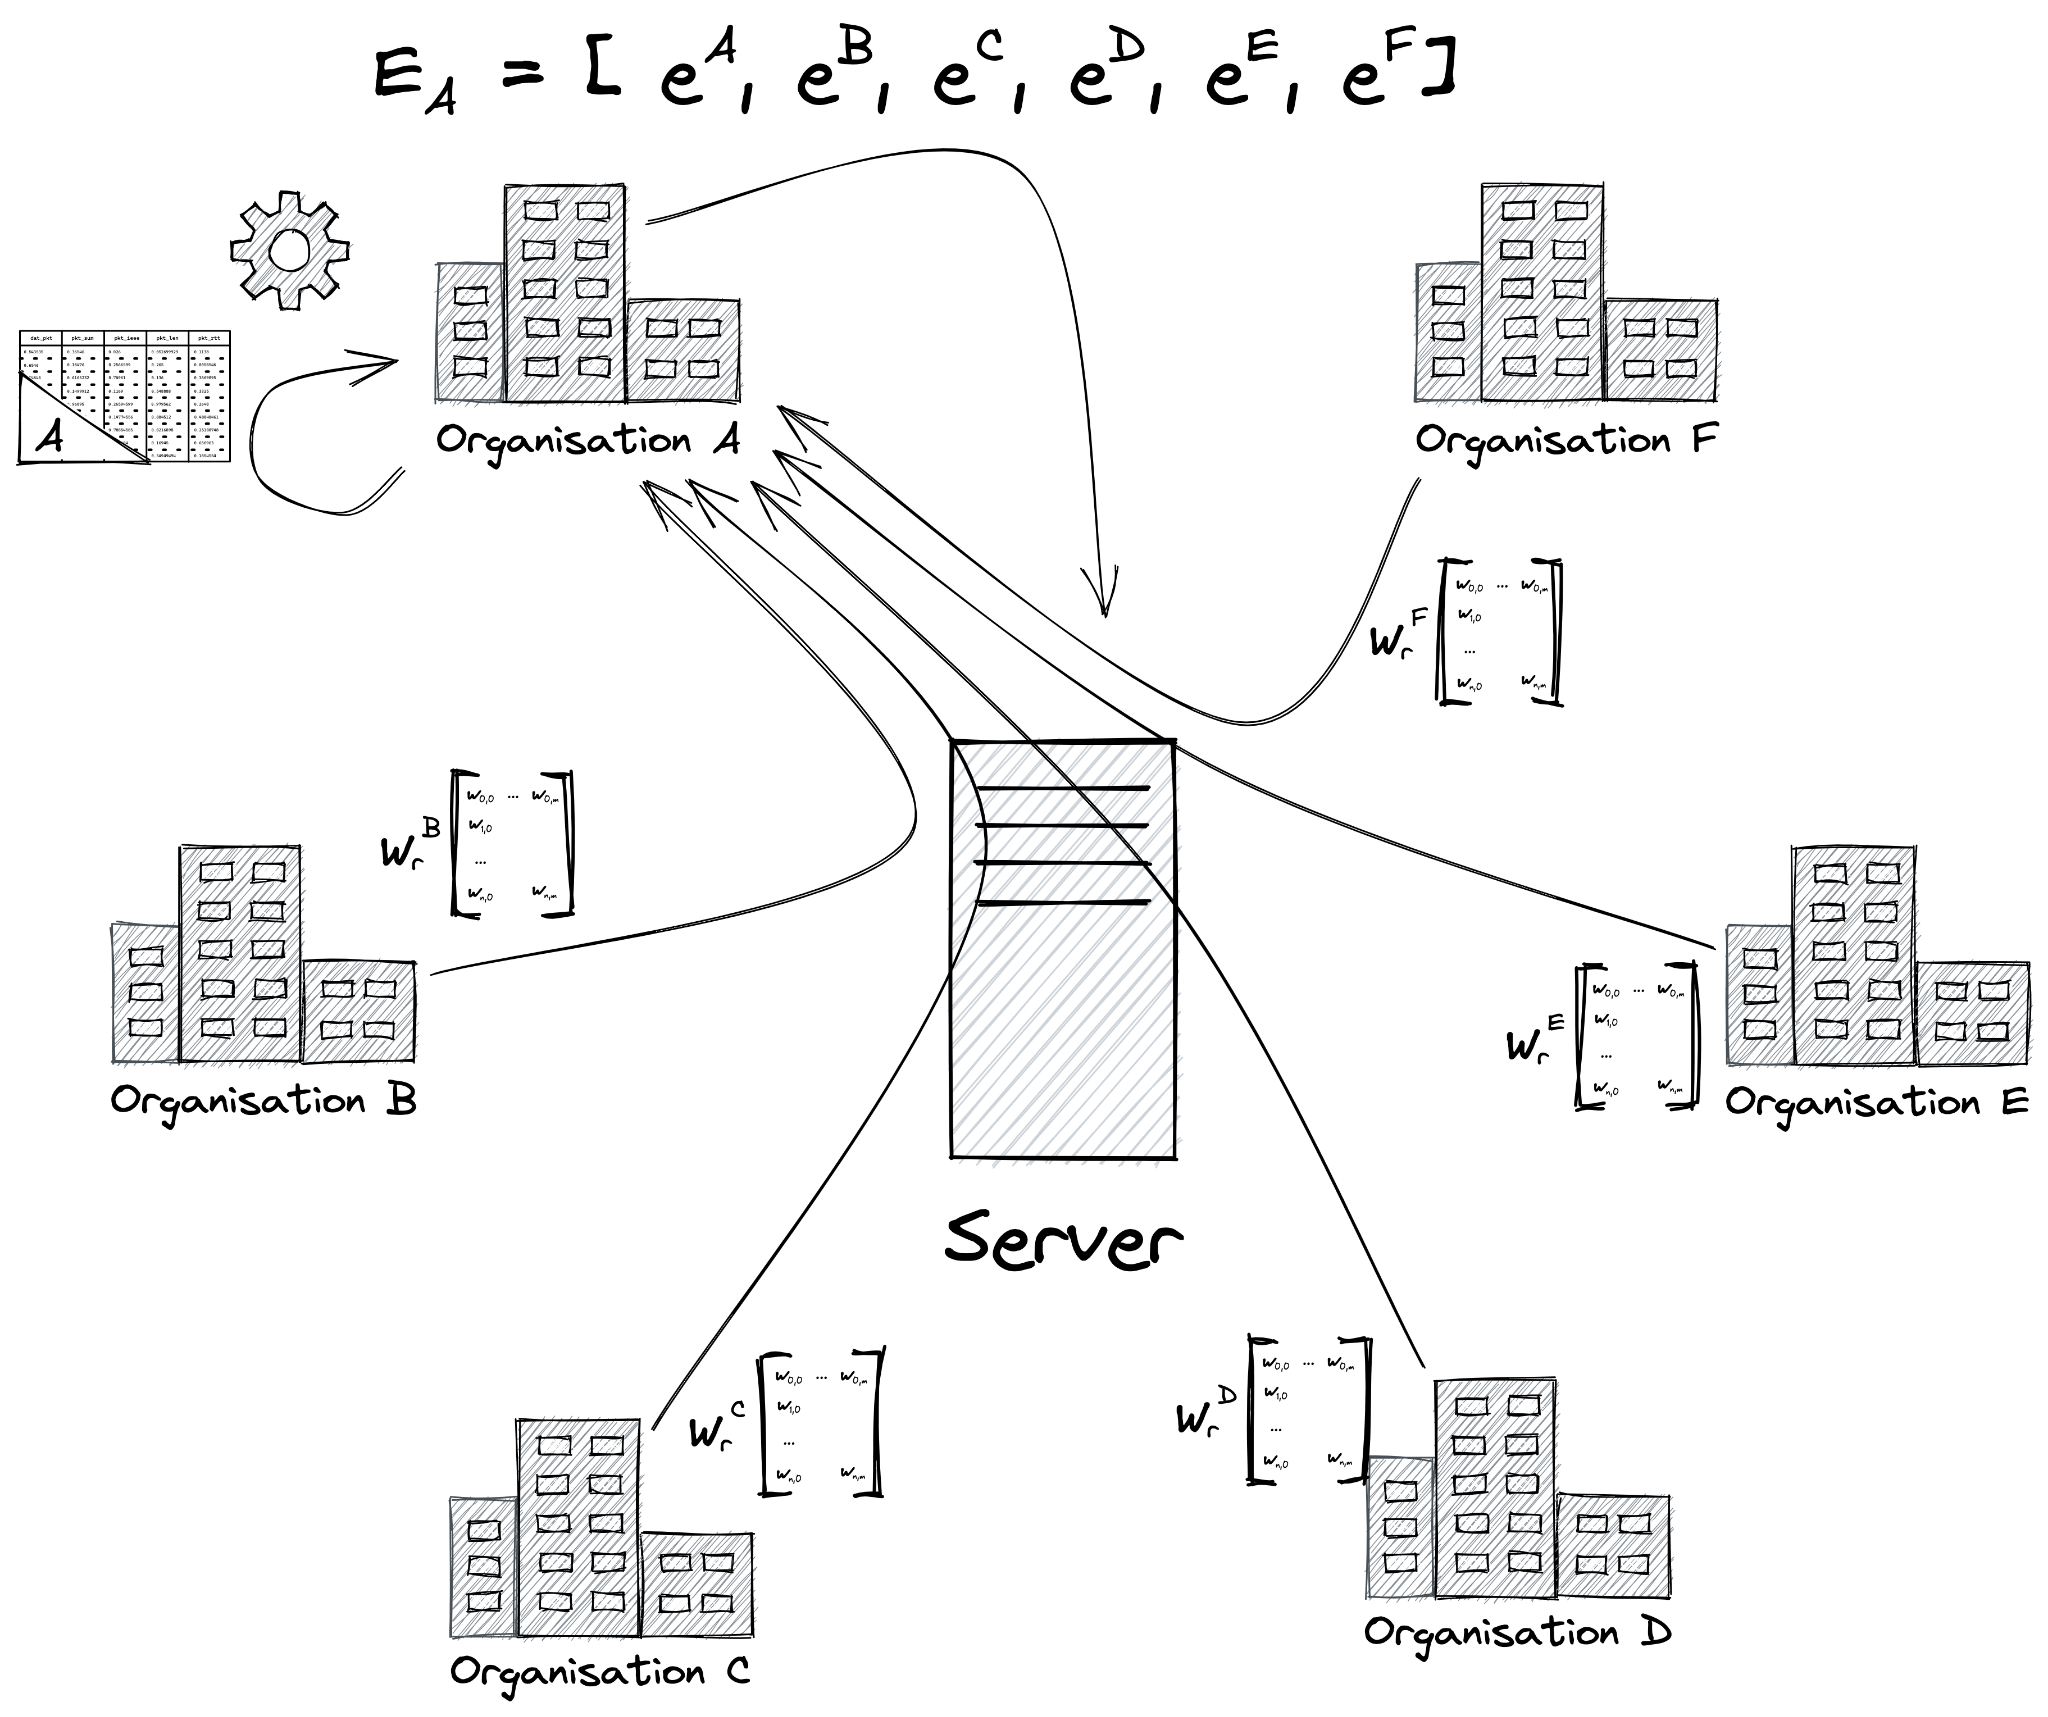
\includegraphics[width=\textwidth]{figures/radar/xeval}
      \end{figure}
    \end{column}
    
    \begin{column}{.55\textwidth}
      \small
      \setlength{\baselineskip}{0.8\baselineskip}
      \vspace{1ex}

      \textbf{Advantages}
      \begin{itemize}
        \item The central server does not need prior knowledge.
        \item Evaluates how each model fits the data (\eg, accuracy, F1 score).
        \item Exhaustive overview of the entire system at each round $r$.
      \end{itemize}

      \pause
      \textbf{Drawbacks}
      \begin{itemize}
        \item High communication and computation costs.
        \item Does not scale well.
        % \item Shares local models to participants: less privacy-friendly.
      \end{itemize}


      \pause
      \textbf{But\dots}
      \begin{itemize}
        \item Cross-silo use case: few clients, with reasonable computing capacity.
        \item Slow workflow: long time between rounds.
      \end{itemize}
    \end{column}

  \end{columns}

\end{frame}

\subsection{Fighting Heterogeneity with Clustering}
% Discours à porter sur cette slide  : 
% Build \emph{more} homogeneous communities of participants to facilitate model aggregation.
% 1 different model per more homogeneous community.
% X-eval results not models : as explained earlier evaluations are representative of participants data distribution. 
\begin{frame}
    \tikz[overlay, remember picture,
      shift=(current page.south west),
      x=(current page.south east),
      y=(current page.north west)
    ]{      
        \node[anchor=south east] at (1,0) {
            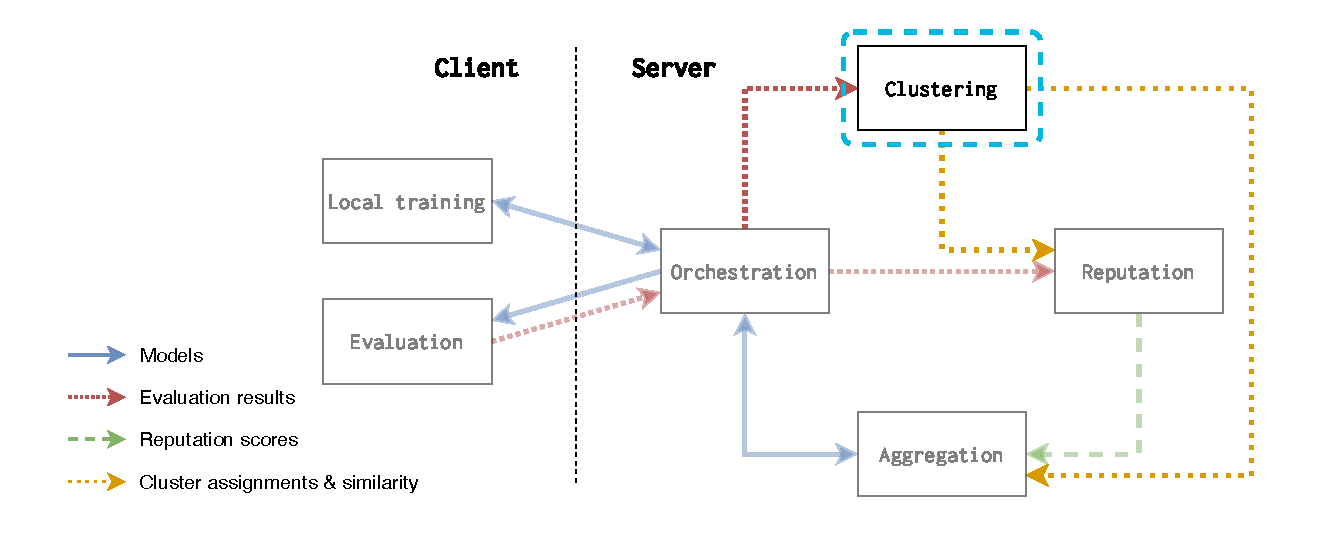
\includegraphics[width=\textwidth]{figures/radar-clust.pdf}
        };
        
        \node[align=left, anchor=north west] at (.05,.91) {\begin{minipage}{.7\textwidth}\subsectionpage\end{minipage}};
    }
\end{frame}
% \begin{frame}{Fighting Heterogeneity with Clustering}
%   % Un ptit graph içi ça ne mangerait pas de pain. 
%   \textbf{Objective}
%   \begin{itemize}
%     \item Build \emph{more} homogeneous communities of participants to facilitate model aggregation.
%   \end{itemize}


%     \pause
%     \textbf{Clustering for FL}\\
%     Leverage cross-evaluation results instead of model updates:
%         \begin{itemize}
%             \item subjective similarity estimation;
%             \item similar evaluations $\rightarrow$ similar data distributions;
%         \end{itemize}
% \end{frame}

\begin{frame}{Fighting Heterogeneity with Clustering}
%Discours :
% Cosine sim : angle measure that will reflect even small changes in a single parameter. 
% Parler du thresold dynamique et de sa méthode de calcul. 
% Exemple rapide du hierarchical clustering.
    \begin{columns}
        \begin{column}{.5\textwidth}
        \begin{itemize}
                \item Distance metric
                \begin{itemize}
                    % \item Between models/gradients;
                    \item Based on \alert{cross-evaluation} results. 
                    \item \alert{Cosine similarity}~\cite{briggs_Federatedlearninghierarchical_2020}.
                \end{itemize}
        \end{itemize}
        \onslide<2->{
            \begin{itemize}
                \item Algorithm
                \begin{itemize}
                    % \item Dynamic \emph{split-and-merge}.~\autocite{chen_ZeroKnowledgeClustering_2021}
                    \item \alert{Hierarchical clustering}.~\autocite{briggs_Federatedlearninghierarchical_2020}
                    \item Dynamic aggregation threshold. 
                \end{itemize}
                \end{itemize}
        }
        \end{column}
        \onslide<2->{
        \begin{column}{.5\textwidth}
            \begin{figure}
                \centering
                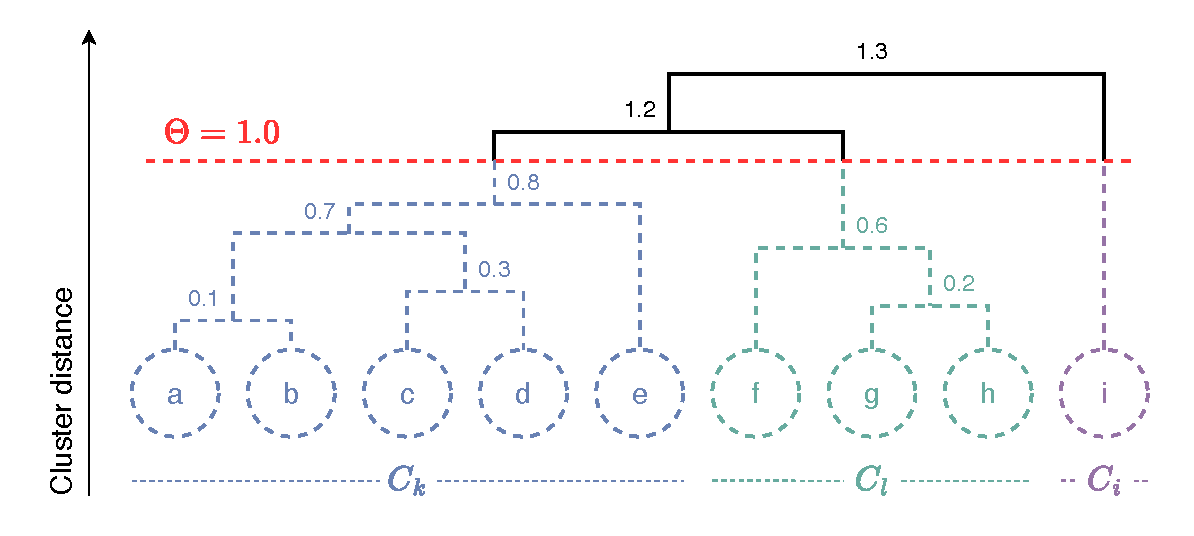
\includegraphics[width=\textwidth]{figures/radar/clustering.drawio.pdf}
                % \makebox[\textwidth][c]{%
                %   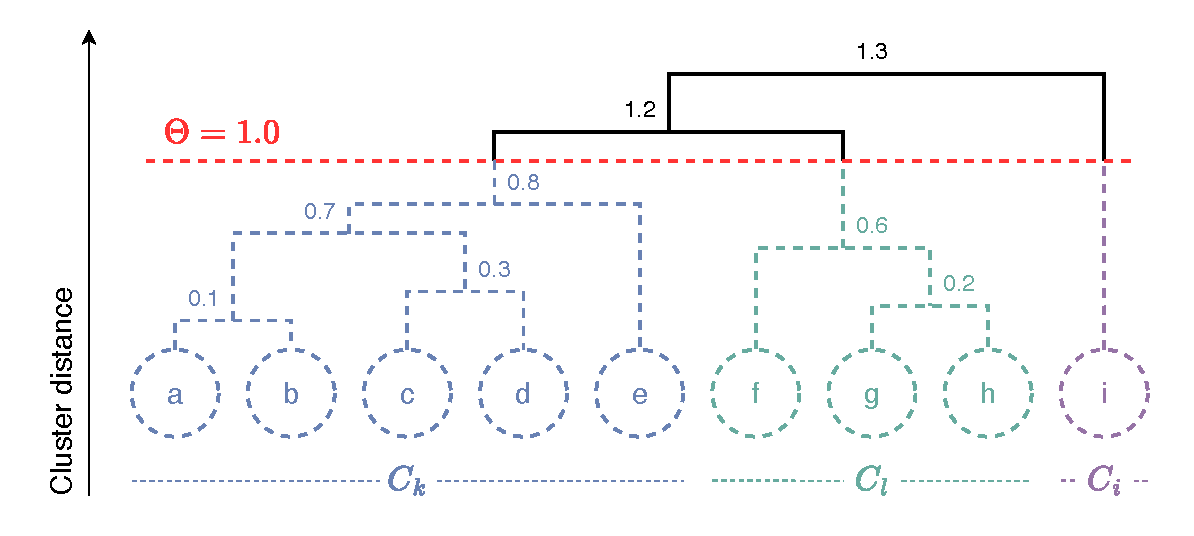
\includegraphics[width=1.2\textwidth]{figures/radar/clustering.drawio.pdf}%
                % }
                \caption{Hierarchical clustering.}
            \end{figure}
        \end{column}
        }
    \end{columns}
    % \only<2->
    \fcitefootnote{briggs_Federatedlearninghierarchical_2020}
    % \fcitefootnote{chen_ZeroKnowledgeClustering_2021}
\end{frame}



\subsection{Mitigating Byzantine Contributions}

\begin{frame}
    \tikz[overlay, remember picture,
      shift=(current page.south west),
      x=(current page.south east),
      y=(current page.north west)
    ]{
        \node[anchor=south east] at (1,0) {
            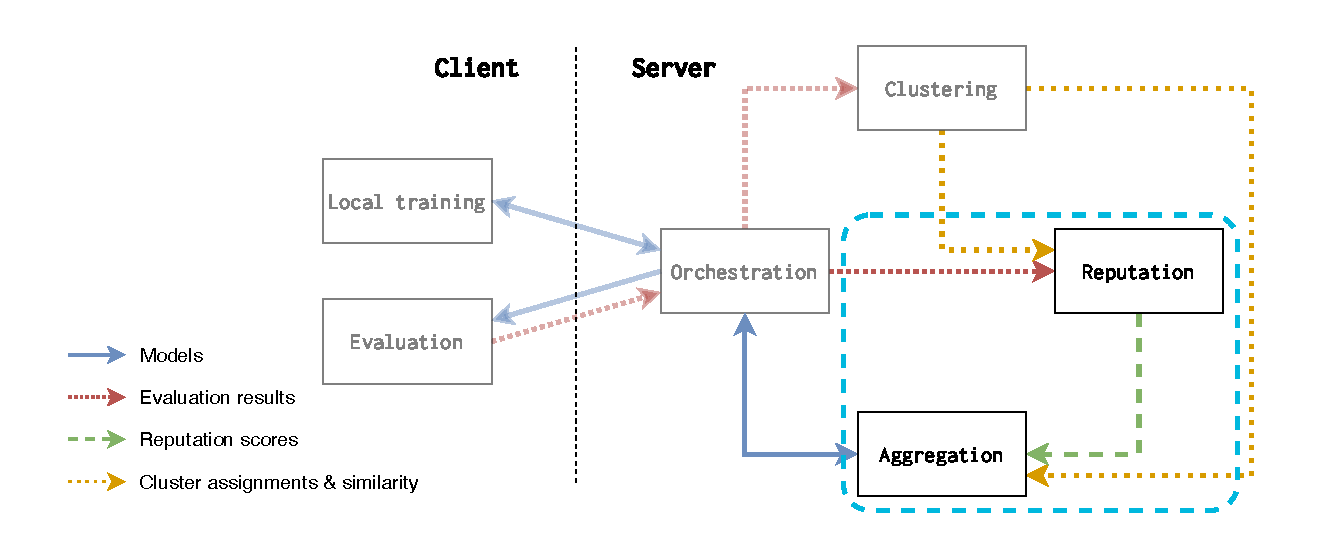
\includegraphics[width=\textwidth]{figures/radar-reput.pdf}
        };
        
        \node[align=left, anchor=north west] at (.05,.91) {\begin{minipage}{.7\textwidth}\subsectionpage\end{minipage}};
    }
\end{frame}
\begin{frame}{Reputation-aware Aggregation}

% Point de discours 
% Déf + pq ça match pour nous.
% On fait de la pondération de modèles plus pertinent pour nous que du choix de modèles.
  \hypersetup{citecolor=.}
  \begin{block}{Definition: Reputation Systems
    \normalfont\autocite{resnick_Reputationsystems_2000}.
    }
    \begin{itemize}
      \item Long-lived entities that inspire an expectation of future interaction;
      \item Capture and distribution of feedback about current interactions (such information must be visible in the future); and
      \item Use of feedback to guide trust decisions.
    \end{itemize}
  \end{block}
 \hypersetup{citecolor=imta-blue}
 
  \onslide<2>{%
    \begin{itemize}
      % \item Dirichlet distribution for local aggregation of the reputation scores.~\autocite{fung_DirichletBasedTrustManagement_2011}
      % \item Votes weighted by the similarity inside each cluster.
      \item Votes weighted based on their similarity to other cluster members. 
      \item Exponential decay to track behavior over time.
    \end{itemize}
  }

  \fcitefootnote{resnick_Reputationsystems_2000}
  % \only<2>{%
  %   \fcitefootnote{fung_DirichletBasedTrustManagement_2011}
  % }

\end{frame}



% Evaluation Setup
% -----------------------------
\section{Evaluation Setup}
\begin{frame}{Experimental Setup}
  \begin{columns}
    \begin{column}{.55\textwidth}
      Similar setup as in the previous case study:
      \begin{itemize}
        \item Heterogeneous datasets, but some participants can share similarities.
        \item 4 datasets: CIC-CSE-IDS2018, UNSW-NB15, Bot-IoT, ToN\_IoT.
        \item NF-V2~\autocite{sarhan_StandardFeatureSet_2021} feature set (\ie, NetFlow V9).
      \end{itemize}
    \end{column}
    \begin{column}{.45\textwidth}
      \begin{figure}

        \includegraphics<1>[height=.5\textheight,left]{figures/radar/distribution.png}%
        \includegraphics<2>[height=.5\textheight,left]{figures/radar/distribution-attack.png}%

        \caption{Distribution of the datasets.}
      \end{figure}
    \end{column}
  \end{columns}
  \fcitefootnote{sarhan_StandardFeatureSet_2021}
\end{frame}


% Results
% -----------------------------
% Results
% -----------------------------
\section{Results}
\begin{frame}{Handling heterogeneity}
  \begin{columns}
    \begin{column}{.4\textwidth}
      \begin{figure}
              \captionsetup{justification=centering}

        % Info à ajouter : RI 1
        % Clustering ok.
        % Animation pour le premier ajout du cercle + le R1 = 1 ? 
        % Indiquer le pourcentage d'empoisonnement en plus. 
        \includegraphics<1>[width=\linewidth,left]{./figures/eval/clustering/clustering_benign.pdf}%
        \caption{Clustering results without poisoning.\\ 
        Rand index=1.0}
      \end{figure}
    \end{column}
  \begin{column}{.6\textwidth}

\begin{table}
    \centering
    % \caption{
    % }
    \footnotesize
    \setlength\tabcolsep{1ex}
    \begin{tabularx}{.7\textwidth}{X|ccc}
      \toprule % ---------------------------------
      \textbf{Scenario}
      & \multicolumn{1}{c}{\texttt{RADAR}} & \multicolumn{1}{c}{\texttt{FG}} & \multicolumn{1}{c|}{\texttt{FC}} \\
      \midrule % ---------------------------------
      \textbf{Benign}& \textbf{0.00} & 5.17 &  0.09  \\
    \end{tabularx}
  \end{table}
  
         \end{column}
  \end{columns}
\end{frame}

%%%%%%%%%%%%
% Untargeted  
%%%%%%%%%%%%
%Lone
%%%%%%%%%%%%
\begin{frame}{Handling untargeted attacks}
  \begin{columns}
    \begin{column}{.4\textwidth}
      \begin{figure}
        \captionsetup{justification=centering}
        % Info à ajouter : RI 1
        % Clustering ok.
        % Animation pour le premier ajout du cercle + le R1 = 1 ? 
        \includegraphics<1>[width=\linewidth,left]{./figures/eval/clustering/clustering_lone_untargeted.pdf}%
        \caption{Clustering results for\\
        \texttt{lone 100U}.\\ 
        Rand index=1.0}
      \end{figure}
    \end{column}
  \begin{column}{.6\textwidth}

\begin{table}
    \centering
    % \caption{
    % }
    \footnotesize
    \setlength\tabcolsep{1ex}
    \begin{tabularx}{.7\textwidth}{lX|ccc}
      \toprule % ---------------------------------
      \multicolumn{2}{c|}{{\textbf{Scenario}}}
      & \multicolumn{1}{c}{\texttt{RADAR}} & \multicolumn{1}{c}{\texttt{FG}} & \multicolumn{1}{c|}{\texttt{FC}} \\
      \midrule % ---------------------------------
      \multicolumn{2}{l|}{\textbf{Benign}}& \textbf{0.00} & 5.17 &  0.09  \\
      % % UNTARGETED ATTACKS
      \multicolumn{2}{l|}{\textbf{Untargeted} (\texttt{100U})}  & & & \\
      & \texttt{Lone} & \textbf{0.08} & 99.89 & 0.12 \\

    \end{tabularx}
  \end{table}
  
         \end{column}
  \end{columns}
\end{frame}

%%%%%%%%%%%%
%Untargeted min bis test1
%%%%%%%%%%%%
\begin{frame}{Handling untargeted attacks. Presentation 1}
  \begin{columns}
    \begin{column}{.4\textwidth}
      \begin{figure}
        \captionsetup{justification=centering}
        % Info à ajouter : RI 1
        % Clustering ok.
        % Animation pour le premier ajout du cercle + le R1 = 1 ? 
        \includegraphics<1>[width=\linewidth,left]{./figures/eval/clustering/clustering_min_untargeted.pdf}%
        \caption{Clustering results for\\ \texttt{colluding minority 100T}\\ 
        Rand index=1.0
        }
      \end{figure}
    \end{column}
  \begin{column}{.6\textwidth}

\begin{table}
    \centering
    % \caption{
    % }
    \footnotesize
    \setlength\tabcolsep{1ex}
    \begin{tabularx}{.7\textwidth}{lX|ccc}
      \toprule % ---------------------------------
      \multicolumn{2}{c|}{{\textbf{Scenario}}}
      & \multicolumn{1}{c}{\texttt{RADAR}} & \multicolumn{1}{c}{\texttt{FG}} & \multicolumn{1}{c|}{\texttt{FC}} \\
      \midrule % ---------------------------------
      \multicolumn{2}{l|}{\textbf{Benign}}& \emoji{green-circle} & \emoji{orange-circle}
 &  \emoji{green-circle}  \\
      % % UNTARGETED ATTACKS
      \multicolumn{2}{l|}{\textbf{Untargeted} (\texttt{100U})}  & & & \\
      & \texttt{Lone} & \emoji{green-circle} & \emoji{red-circle} & \emoji{green-circle} \\
      & \texttt{Collud. min.} &  \emoji{green-circle} & \emoji{green-circle} & \emoji{orange-circle}
 \\
    \end{tabularx}
  \end{table}
  
         \end{column}
  \end{columns}
\end{frame}

%%%%%%%%%%%%
%Untargeted min bis test2
%%%%%%%%%%%%
\begin{frame}{Handling untargeted attacks. Presentation 2}
  \begin{columns}
    \begin{column}{.4\textwidth}
      \begin{figure}
        \captionsetup{justification=centering}
        % Info à ajouter : RI 1
        % Clustering ok.
        % Animation pour le premier ajout du cercle + le R1 = 1 ? 
        \includegraphics<1>[width=\linewidth,left]{./figures/eval/clustering/clustering_min_untargeted.pdf}%
        \caption{Clustering results for\\ \texttt{colluding minority 100T}\\ 
        Rand index=1.0
        }
      \end{figure}
    \end{column}
  \begin{column}{.6\textwidth}

\begin{table}
    \centering
    % \caption{
    % }
    \footnotesize
    \setlength\tabcolsep{1ex}
    \begin{tabularx}{.7\textwidth}{lX|ccc}
      \toprule % ---------------------------------
      \multicolumn{2}{c|}{{\textbf{Scenario}}}
      & \multicolumn{1}{c}{\texttt{RADAR}} & \multicolumn{1}{c}{\texttt{FG}} & \multicolumn{1}{c|}{\texttt{FC}} \\
      \midrule % ---------------------------------
      \multicolumn{2}{l|}{\textbf{Benign}}& \hg \textbf{0.00} & \ho 5.17 & \hg 0.09  \\
      % % UNTARGETED ATTACKS
      \multicolumn{2}{l|}{\textbf{Untargeted} (\texttt{100U})}  & & & \\
      % & \texttt{Benign} &  0.09  & 0.39 & 33.30 & \textbf{0.06} \\
      & \texttt{Lone} & \hg \textbf{0.08} &\hr 99.89 & \hg 0.12 \\
      & \texttt{Collud. min.} & \hg 0.10 & \hg \textbf{0.04} &\ho 6.26 \\
    \end{tabularx}
  \end{table}
  
         \end{column}
  \end{columns}
\end{frame}


%%%%%%%%%%%%
%Untargeted min
%%%%%%%%%%%%
\begin{frame}{Handling untargeted attacks}
  \begin{columns}
    \begin{column}{.4\textwidth}
      \begin{figure}
        \captionsetup{justification=centering}
        % Info à ajouter : RI 1
        % Clustering ok.
        % Animation pour le premier ajout du cercle + le R1 = 1 ? 
        \includegraphics<1>[width=\linewidth,left]{./figures/eval/clustering/clustering_min_untargeted.pdf}%
        \caption{Clustering results for\\ \texttt{colluding minority 100T}\\ 
        Rand index=1.0
        }
      \end{figure}
    \end{column}
  \begin{column}{.6\textwidth}

\begin{table}
    \centering
    % \caption{
    % }
    \footnotesize
    \setlength\tabcolsep{1ex}
    \begin{tabularx}{.7\textwidth}{lX|ccc}
      \toprule % ---------------------------------
      \multicolumn{2}{c|}{{\textbf{Scenario}}}
      & \multicolumn{1}{c}{\texttt{RADAR}} & \multicolumn{1}{c}{\texttt{FG}} & \multicolumn{1}{c|}{\texttt{FC}} \\
      \midrule % ---------------------------------
      \multicolumn{2}{l|}{\textbf{Benign}}& \textbf{0.00} & 5.17 &  0.09  \\
      % % UNTARGETED ATTACKS
      \multicolumn{2}{l|}{\textbf{Untargeted} (\texttt{100U})}  & & & \\
      % & \texttt{Benign} &  0.09  & 0.39 & 33.30 & \textbf{0.06} \\
      & \texttt{Lone} & \textbf{0.08} & 99.89 & 0.12 \\
      & \texttt{Collud. min.} &  0.10 & \textbf{0.04} & 6.26 \\
    \end{tabularx}
  \end{table}
  
         \end{column}
  \end{columns}
\end{frame}


%%%%%%%%%%%%
%Untargeted maj
%%%%%%%%%%%%
\begin{frame}{Handling untargeted attacks}
  \begin{columns}
    \begin{column}{.4\textwidth}
      \begin{figure}
        \captionsetup{justification=centering}
        % Info à ajouter : RI 1
        % Clustering ok.
        % Animation pour le premier ajout du cercle + le R1 = 1 ? 
        \includegraphics<1>[width=\linewidth,left]{./figures/eval/clustering/clustering_maj_untargeted.pdf}%
        \caption{Clustering results for\\
        \texttt{colluding majority 100U}\\ 
        Rand index=1.0}
      \end{figure}
    \end{column}
  \begin{column}{.6\textwidth}

\begin{table}
    \centering
    % \caption{
    % }
    \footnotesize
    \setlength\tabcolsep{1ex}
    \begin{tabularx}{.7\textwidth}{lX|ccc}
      \toprule % ---------------------------------
      \multicolumn{2}{c|}{{\textbf{Scenario}}}
      & \multicolumn{1}{c}{\texttt{RADAR}} & \multicolumn{1}{c}{\texttt{FG}} & \multicolumn{1}{c|}{\texttt{FC}} \\
      \midrule % ---------------------------------
      \multicolumn{2}{l|}{\textbf{Benign}}& \textbf{0.00} & 5.17 &  0.09  \\
      % % UNTARGETED ATTACKS
      \multicolumn{2}{l|}{\textbf{Untargeted} (\texttt{100U})}  & & & \\
      % & \texttt{Benign} &  0.09  & 0.39 & 33.30 & \textbf{0.06} \\
      & \texttt{Lone} & \textbf{0.08} & 99.89 & 0.12 \\
      & \texttt{Collud. min.} &  0.10 & \textbf{0.04} & 6.26 \\
      & \texttt{Collud. maj.} &  \textbf{0.08} & 38.98 & 94.36 \\                  % TARGETED ATTACKS
 
                  % & \texttt{Lone} &  \textbf{0.00} & 93.82 & 6.73 &  0.45 \\
                  % & \texttt{Collud. min.} &  \textbf{0.00} &  2.97 & 9.99 & 53.40 \\
                  % & \texttt{Collud. maj.} &  73.39 & \textbf{8.10} & 17.65 & 59.36 \\
      % \midrule % ---------------------------------
          
      % \bottomrule % ---------------------------------
      % \small & \multicolumn{1}{c}{} & \multicolumn{4}{c}{\emph{lower is better}}
    \end{tabularx}
  \end{table}
  
         \end{column}
  \end{columns}
\end{frame}


%%%%%%%%%%%%    
% Targeted   
%%%%%%%%%%%%
%%%%%%%%%%%%    
% Lone   
%%%%%%%%%%%%
\begin{frame}{Handling targeted attacks: clustering effect}
  \begin{columns}
    \begin{column}{.4\textwidth}
      \begin{figure}
        \captionsetup{justification=centering}
        % Info à ajouter : RI 1
        % Clustering ok.
        % Animation pour le premier ajout du cercle + le R1 = 1 ? 
        \includegraphics<1>[width=\linewidth,left]{./figures/eval/clustering/clustering_lone_targeted.pdf}%
        \caption{Clustering results for\\
        \texttt{Lone 100T}\\ 
        Rand index=0.97}
      \end{figure}
    \end{column}
  \begin{column}{.6\textwidth}
                \begin{table}
                    \centering
                    \footnotesize
                    \setlength\tabcolsep{1ex}
                        \begin{tabularx}{.7\textwidth}{lX|ccc}
                            \toprule % ---------------------------------
                            \multicolumn{2}{c|}{{\textbf{Scenario}}}
                            & \multicolumn{1}{c}{\texttt{RADAR}} & \multicolumn{1}{c}{\texttt{FG}} & \multicolumn{1}{c|}{\texttt{FC}} \\
                            \midrule % ---------------------------------
                            \multicolumn{2}{l|}{\textbf{Benign}}& \textbf{0.00} & 5.17 &  0.09  \\
                            % % TARGETED ATTACKS
                            \multicolumn{2}{l|}{\textbf{Targeted} (\texttt{100T})}  & & & \\    
                            & \texttt{Lone} &\tikz[baseline]{ \node[anchor=base] (t1){\textbf{0.00}}}  & 93.82 &  0.45 \\
                        \end{tabularx}
                \end{table}
                  
                % Still, the results are good, why ? 
                % \tikz[na]\node [coordinate] (n2) {};
                
                % \begin{tikzpicture}[overlay]
                %     \path[->]<1-> (n1) edge [bend right] (t1);
                % \end{tikzpicture}

         \end{column}
  \end{columns}
\end{frame}

%%%%%%%%%%%%    
% Lone bis 
%%%%%%%%%%%%
\begin{frame}{Handling targeted attacks: reputation effect}
  \begin{columns}
    \begin{column}{.4\textwidth}
      \begin{figure}
        \captionsetup{justification=centering}
        % Info à ajouter : RI 1
        % Clustering ok.
        % Animation pour le premier ajout du cercle + le R1 = 1 ? 
        \includegraphics<1>[width=\linewidth,left]{./figures/eval/clustering/clustering_lone_targeted.pdf}%
        \caption{Clustering results for\\
        \texttt{Lone 100T}\\ 
        Rand index=0.97}
      \end{figure}
    \end{column}
  \begin{column}{.6\textwidth}

  \begin{minipage}[t][0.35\textheight]{\textwidth}
                \centering
                \begin{table}
                    \centering
                    \footnotesize
                    \setlength\tabcolsep{1ex}
                        \begin{tabularx}{.7\textwidth}{lX|ccc}
                            \toprule % ---------------------------------
                            \multicolumn{2}{c|}{{\textbf{Scenario}}}
                            & \multicolumn{1}{c}{\texttt{RADAR}} & \multicolumn{1}{c}{\texttt{FG}} & \multicolumn{1}{c|}{\texttt{FC}} \\
                            \midrule % ---------------------------------
                            \multicolumn{2}{l|}{\textbf{Benign}}& \textbf{0.00} & 5.17 &  0.09  \\
                            % % TARGETED ATTACKS
                            \multicolumn{2}{l|}{\textbf{Targeted} (\texttt{100T})}  & & & \\    
                            & \texttt{Lone} &\textbf{0.00} & 93.82 &  0.45 \\
                        \end{tabularx}
                \end{table}
        \end{minipage}
        % \vspace{0.25cm}            
    \begin{minipage}[t][0.65\textheight]{\textwidth}
        \begin{figure}
        % Matérialiser le zoom du cluster rouge vers les courbes de droites ?  
            \captionsetup{justification=centering}
                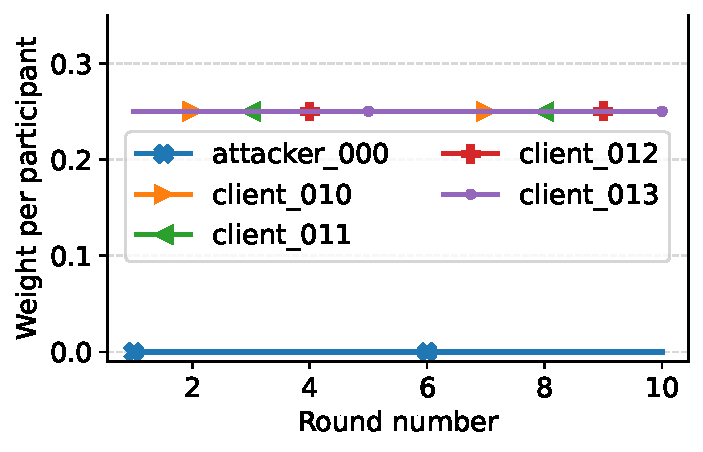
\includegraphics[width=0.65\linewidth]{./figures/eval/reput/lone_loud_expanded.pdf}
                \caption{Participants reputation for\\
                \texttt{Lone 100T}}
      \end{figure}
    \end{minipage}  
  
    \end{column}
  \end{columns}
\end{frame}


%%%%%%%%%%%%    
% Targeted min   
%%%%%%%%%%%%
\begin{frame}{Handling targeted attacks}
  \begin{columns}
    \begin{column}{.4\textwidth}
      \begin{figure}
        \captionsetup{justification=centering}
        % Info à ajouter : RI 1
        % Clustering ok.
        % Animation pour le premier ajout du cercle
        \includegraphics<1>[width=\linewidth,left]{./figures/eval/clustering/clustering_min_targeted.pdf}%
        \caption{Clustering results for\\
        \texttt{colluding minority 100T}\\ 
        Rand index=0.97}
      \end{figure}
    \end{column}
  \begin{column}{.6\textwidth}

\begin{table}
    \centering
    % \caption{
    % }
    \footnotesize
    \setlength\tabcolsep{1ex}
    \begin{tabularx}{.7\textwidth}{lX|ccc}
      \toprule % ---------------------------------
      \multicolumn{2}{c|}{{\textbf{Scenario}}}
      & \multicolumn{1}{c}{\texttt{RADAR}} & \multicolumn{1}{c}{\texttt{FG}} & \multicolumn{1}{c|}{\texttt{FC}} \\
      \midrule % ---------------------------------
      \multicolumn{2}{l|}{\textbf{Benign}}& \textbf{0.00} & 5.17 &  0.09  \\
      % % TARGETED ATTACKS
      \multicolumn{2}{l|}{\textbf{Targeted} (\texttt{100T})}  & & & \\                  
                  & \texttt{Lone} &  \textbf{0.00} & 93.82 &  0.45 \\
                  & \texttt{Collud. min.} &  \textbf{0.00} &  2.97 & 53.40 \\
%                   % & \texttt{Collud. maj.} &  73.39 & \textbf{8.10} & 59.36 \\

    \end{tabularx}
  \end{table}
  
         \end{column}
  \end{columns}
\end{frame}
%%%%%%%%%%%%    
% Targeted maj   
%%%%%%%%%%%%
\begin{frame}{Handling targeted attacks}
  \begin{columns}
    \begin{column}{.4\textwidth}
      \begin{figure}
        \captionsetup{justification=centering}
        % Info à ajouter : RI 1
        % Clustering ok.
        % Animation pour le premier ajout du cercle + le R1 = 1 ? 
        \includegraphics<1>[width=\linewidth,left]{./figures/eval/clustering/clustering_maj_targeted.pdf}%
        \caption{Clustering results for \texttt{colluding majority 100T}\\ 
        Rand index=0.96}
      \end{figure}
    \end{column}
  \begin{column}{.6\textwidth}

\begin{table}
    \centering
    % \caption{
    % }
    \footnotesize
    \setlength\tabcolsep{1ex}
    \begin{tabularx}{.7\textwidth}{lX|ccc}
      \toprule % ---------------------------------
      \multicolumn{2}{c|}{{\textbf{Scenario}}}
      & \multicolumn{1}{c}{\texttt{RADAR}} & \multicolumn{1}{c}{\texttt{FG}} & \multicolumn{1}{c|}{\texttt{FC}} \\
      \midrule % ---------------------------------
      \multicolumn{2}{l|}{\textbf{Benign}}& \textbf{0.00} & 5.17 &  0.09  \\
      % % TARGETED ATTACKS
      \multicolumn{2}{l|}{\textbf{Targeted} (\texttt{100T})}  & & & \\                  
                  & \texttt{Lone} &  \textbf{0.00} & 93.82 &  0.45 \\
                  & \texttt{Collud. min.} &  \textbf{0.00} &  2.97 & 53.40 \\
                  & \texttt{Collud. maj.} &  73.39 & \textbf{8.10} & 59.36 \\

    \end{tabularx}
  \end{table}
  
         \end{column}
  \end{columns}
\end{frame}


%% Dummy frame 
% \section{Results}
% \begin{frame}{Handling heterogeneity}
%   \begin{columns}
%     \begin{column}{.4\textwidth}
%       \begin{figure}
%         % Info à ajouter : RI 1
%         % Clustering ok.
%         % Animation pour le premier ajout du cercle + le R1 = 1 ? 
%         \includegraphics<1>[width=\linewidth,left]{./figures/eval/clustering_untargeted_min.pdf}%
%         \caption{Clustering results without poisoning.}
%       \end{figure}
%     \end{column}
%   \begin{column}{.6\textwidth}

% \begin{table}
%     \centering
%     % \caption{
%     % }
%     \footnotesize
%     \setlength\tabcolsep{1ex}
%     \begin{tabularx}{.7\textwidth}{lX|ccc}
%       \toprule % ---------------------------------
%       \multicolumn{2}{c|}{{\textbf{Scenario}}}
%       & \multicolumn{1}{c}{\texttt{RADAR}} & \multicolumn{1}{c}{\texttt{FG}} & \multicolumn{1}{c|}{\texttt{FC}} \\
%       \midrule % ---------------------------------
%       \multicolumn{2}{l|}{\textbf{Benign}}& \textbf{0.00} & 5.17 &  0.09  \\

%       % TARGETED ATTACKS
%       % \multicolumn{2}{l|}{\textbf{Targeted} (\texttt{100U})}  & & & \\                  
%                   % & \texttt{Lone} &  \textbf{0.00} & 93.82 & 6.73 &  0.45 \\
%                   % & \texttt{Collud. min.} &  \textbf{0.00} &  2.97 & 9.99 & 53.40 \\
%                   % & \texttt{Collud. maj.} &  73.39 & \textbf{8.10} & 17.65 & 59.36 \\
%       % \midrule % ---------------------------------
%       % % UNTARGETED ATTACKS
%       % \multicolumn{2}{l|}{\textbf{Untargeted} (\texttt{100U})}  & & & \\
%       % & \texttt{Benign} &  0.09  & 0.39 & 33.30 & \textbf{0.06} \\
%       % & \texttt{Lone} & \textbf{0.08} & 99.89 & 54.70 & 0.12 \\
%       % & \texttt{Collud. min.} &  0.10 & \textbf{0.04} & 44.53 & 6.26 \\
%       % & \texttt{Collud. maj.} &  \textbf{0.08} & 38.98 & 59.49 & 94.36 \\          
%       % \bottomrule % ---------------------------------
%       % \small & \multicolumn{1}{c}{} & \multicolumn{4}{c}{\emph{lower is better}}
%     \end{tabularx}
%   \end{table}
  
%          \end{column}
%   \end{columns}
% \end{frame}



% Conclusion
% -----------------------------
\section*{Conclusion}

\begin{frame}
  \sectionpage
\end{frame}

\begin{frame}{Fighting Byzantine Attacks in Federated Learning}
  \textbf{The proposed framework can:}
  \begin{itemize}
    \item Leverage cross evaluation, clustering and reputation to address heterogeneity and poisoning.  
    \item Adjust rapidly to changes in behavior.  
    \item Mitigate most tested scenarios. Only one, limit case on colluding targeted attackers poisoning more than 80\% of their data. 
  \end{itemize}


  \pause
  \textbf{How generic?}
  \begin{itemize}
    \item Only few conditions: parametric models, locally owned evaluation set, a \alert<3>{small-scale use case}, and a \alert<3>{trusted central server}.
  \end{itemize}
\end{frame}


\begin{frame}{Future Work}
  \textbf{Future works:}
    \begin{itemize}
      \item Remove the central server dependency.
      \item Reduce the cross-evaluation overhead to extend applicability to cross device settings.
      \item Test the approach in more realistic heterogeneous settings.
    \end{itemize}
\end{frame}


\begin{frame}
  \centering\scshape\large Thank you for your attention!

  \vfill
  
  \normalshape\normalsize

  % \textbf{RADAR: Model Quality Assessment for Reputation-aware\\ Collaborative Federated Learning}
  % \medskip
  
  \raggedright
  \begin{itemize}
    \item A novel architecture for cross-silo FL, combining reputation and clustering to ensure model quality.
    % \item An evaluation showing great coverage in the mitigated scenarios.
    \item An evaluation highlighting \texttt{RADAR} resilience against a great range of failure and attack scenarios.
    \item Promising research directions towards trustable, decentralized, privacy-preserving collaborative learning.
  \end{itemize}

  \vfill

  \centering\small
  leo.lavaur@imt-atlantique.fr\\
  pierre-marie.lechevalier@imt-atlantique.fr

\end{frame}




% Backup Slides
% -----------------------------
%
\section*{Extra Slides}

\begin{frame}
  \sectionpage
\end{frame}

\begin{frame}{Results}
  \begin{table}
    \centering
    \caption{
      \emph{Effect of different attack configurations (untargeted) on all baselines.}
      \texttt{RA} is RADAR, \texttt{FG} is \texttt{FoolsGold}, \texttt{FA} is \texttt{FedAvg} (on \emph{all} participants), and \texttt{FC} is \texttt{FedAvg} ideally clustered per dataset.
    }

    \footnotesize

    \newcommand{\hl}{}
    \only<2>{\renewcommand{\hl}{\cellcolor{imta-green!30}}}


  
    \setlength\tabcolsep{1ex}
    \begin{tabularx}{.8\textwidth}{lX|rrrr|rrrr}
      \toprule % ---------------------------------
      \multicolumn{2}{c|}{\multirow{2}{*}{\textbf{Scenario}}} & \multicolumn{4}{c|}{\textbf{Mean accuracy} (\%)} & \multicolumn{4}{c}{\textbf{\gls{asr}} (\%)} \\
      & & \multicolumn{1}{c}{\texttt{RA}} & \multicolumn{1}{c}{\texttt{FG}} & \multicolumn{1}{c}{\texttt{FA}} & \multicolumn{1}{c|}{\texttt{FC}} & \multicolumn{1}{c}{\texttt{RA}} & \multicolumn{1}{c}{\texttt{FG}} & \multicolumn{1}{c}{\texttt{FA}} & \multicolumn{1}{c}{\texttt{FC}} \\
      \midrule % ---------------------------------
      % TARGETED ATTACKS
      \multicolumn{2}{l|}{\textbf{Targeted} (\texttt{100T})} & & & & & & & & \\
                  & \texttt{Benign}       & \hl 99.07 & 55.04 & 79.49 & \textbf{99.24} & \hl \textbf{0.00} &  5.17 & 5.10 &  0.09 \\
                  & \texttt{Lone}         & \hl 99.06 & 60.51 & 77.38 & \textbf{99.22} & \hl \textbf{0.00} & 93.82 & 6.73 &  0.45 \\
                  & \texttt{Collud. min.} & \hl \textbf{98.96} & 54.64 & 78.48 & 98.33 & \hl \textbf{0.00} &  2.97 & 9.99 & 53.40 \\
                  & \texttt{Collud. maj.} & \hl \textbf{98.28} & 85.10 & 79.40 & 98.22 & \hl \only<3>{\bfseries\color{red}} 73.39 & \textbf{8.10} & 17.65 & 59.36 \\
      \midrule % ---------------------------------
      % UNTARGETED ATTACKS
      \multicolumn{2}{l|}{\textbf{Untargeted} (\texttt{100U})} & & & & & & & & \\
      & \texttt{Benign}        & \hl 99.07 & 55.04 & 79.49 & \textbf{99.24} & \hl 0.09  & 0.39 & 33.30 & \textbf{0.06} \\
      & \texttt{Lone}          & \hl 98.96 & 49.56 & 78.38 & \textbf{99.22} &\hl \textbf{0.08} & 99.89 & 54.70 & 0.12 \\
      & \texttt{Collud. min.}  & \hl \textbf{98.98} & 49.67 & 72.47 & 97.69 & \hl 0.10 & \textbf{0.04} & 44.53 & 6.26 \\
      & \texttt{Collud. maj.}  & \hl \textbf{98.96} & 69.09 & 81.87 & 75.66 & \hl \textbf{0.08} & 38.98 & 59.49 & 94.36 \\          
      \bottomrule % ---------------------------------
      \small & \multicolumn{1}{c}{} & \multicolumn{4}{c}{\emph{higher is better}} & \multicolumn{4}{c}{\emph{lower is better}}
    \end{tabularx}
  \end{table}
  
\end{frame}

\begin{frame}{Results}
  \begin{table}
    \centering
    \caption{
      \emph{Effect of different attack configurations (untargeted) on all baselines.}
      \texttt{RA} is RADAR, \texttt{FG} is \texttt{FoolsGold}, \texttt{FA} is \texttt{FedAvg} (on \emph{all} participants), and \texttt{FC} is \texttt{FedAvg} ideally clustered per dataset.
    }

    \footnotesize

    \newcommand{\hl}{}
    \only<2>{\renewcommand{\hl}{\cellcolor{imta-green!30}}}


  
    \setlength\tabcolsep{1ex}
    \begin{tabularx}{.8\textwidth}{lX|rrrr|rrrr}
      \toprule % ---------------------------------
      \multicolumn{2}{c|}{\multirow{2}{*}{\textbf{Scenario}}} & \multicolumn{4}{c|}{\textbf{Mean accuracy} (\%)} & \multicolumn{4}{c}{\textbf{\gls{asr}} (\%)} \\
      & & \multicolumn{1}{c}{\texttt{RA}} & \multicolumn{1}{c}{\texttt{FG}} & \multicolumn{1}{c}{\texttt{FA}} & \multicolumn{1}{c|}{\texttt{FC}} & \multicolumn{1}{c}{\texttt{RA}} & \multicolumn{1}{c}{\texttt{FG}} & \multicolumn{1}{c}{\texttt{FA}} & \multicolumn{1}{c}{\texttt{FC}} \\
      \midrule % ---------------------------------
      % TARGETED ATTACKS
      \multicolumn{2}{l|}{\textbf{Targeted} (\texttt{100T})} & & & & & & & & \\
                  & \texttt{Benign}       & \hl 99.07 & 55.04 & 79.49 & \textbf{99.24} & \hl \textbf{0.00} &  5.17 & 5.10 &  0.09 \\
                  & \texttt{Lone}         & \hl 99.06 & 60.51 & 77.38 & \textbf{99.22} & \hl \textbf{0.00} & 93.82 & 6.73 &  0.45 \\
                  & \texttt{Collud. min.} & \hl \textbf{98.96} & 54.64 & 78.48 & 98.33 & \hl \textbf{0.00} &  2.97 & 9.99 & 53.40 \\
                  & \texttt{Collud. maj.} & \hl \textbf{98.28} & 85.10 & 79.40 & 98.22 & \hl \only<3>{\bfseries\color{red}} 73.39 & \textbf{8.10} & 17.65 & 59.36 \\
      \midrule % ---------------------------------
      % UNTARGETED ATTACKS
      \multicolumn{2}{l|}{\textbf{Untargeted} (\texttt{100U})} & & & & & & & & \\
      & \texttt{Benign}        & \hl 99.07 & 55.04 & 79.49 & \textbf{99.24} & \hl 0.09  & 0.39 & 33.30 & \textbf{0.06} \\
      & \texttt{Lone}          & \hl 98.96 & 49.56 & 78.38 & \textbf{99.22} &\hl \textbf{0.08} & 99.89 & 54.70 & 0.12 \\
      & \texttt{Collud. min.}  & \hl \textbf{98.98} & 49.67 & 72.47 & 97.69 & \hl 0.10 & \textbf{0.04} & 44.53 & 6.26 \\
      & \texttt{Collud. maj.}  & \hl \textbf{98.96} & 69.09 & 81.87 & 75.66 & \hl \textbf{0.08} & 38.98 & 59.49 & 94.36 \\          
      \bottomrule % ---------------------------------
      \small & \multicolumn{1}{c}{} & \multicolumn{4}{c}{\emph{higher is better}} & \multicolumn{4}{c}{\emph{lower is better}}
    \end{tabularx}
  \end{table}
  
\end{frame}
\begin{frame}{Intrusion Detection}
  
  \textbf{Machine Learning (ML) for Network-based Intrusion Detection Systems (NIDSs)}
  \begin{itemize}
    \item Detect \alert{malicious} activities (\ie, \textit{misuse detection}) or \alert{anomalies} (\ie, \textit{anomaly detection}).
    \item Various types of algorithms: \alert<2>{supervised}, unsupervised, semi-supervised, reinforcement learning, \textit{etc}.
    \item Great performance with Deep Learning (DL) (on public datasets at least).
  \end{itemize}
  \bigskip
    
  \begin{figure}
    \centering
    \makebox[\textwidth][c]{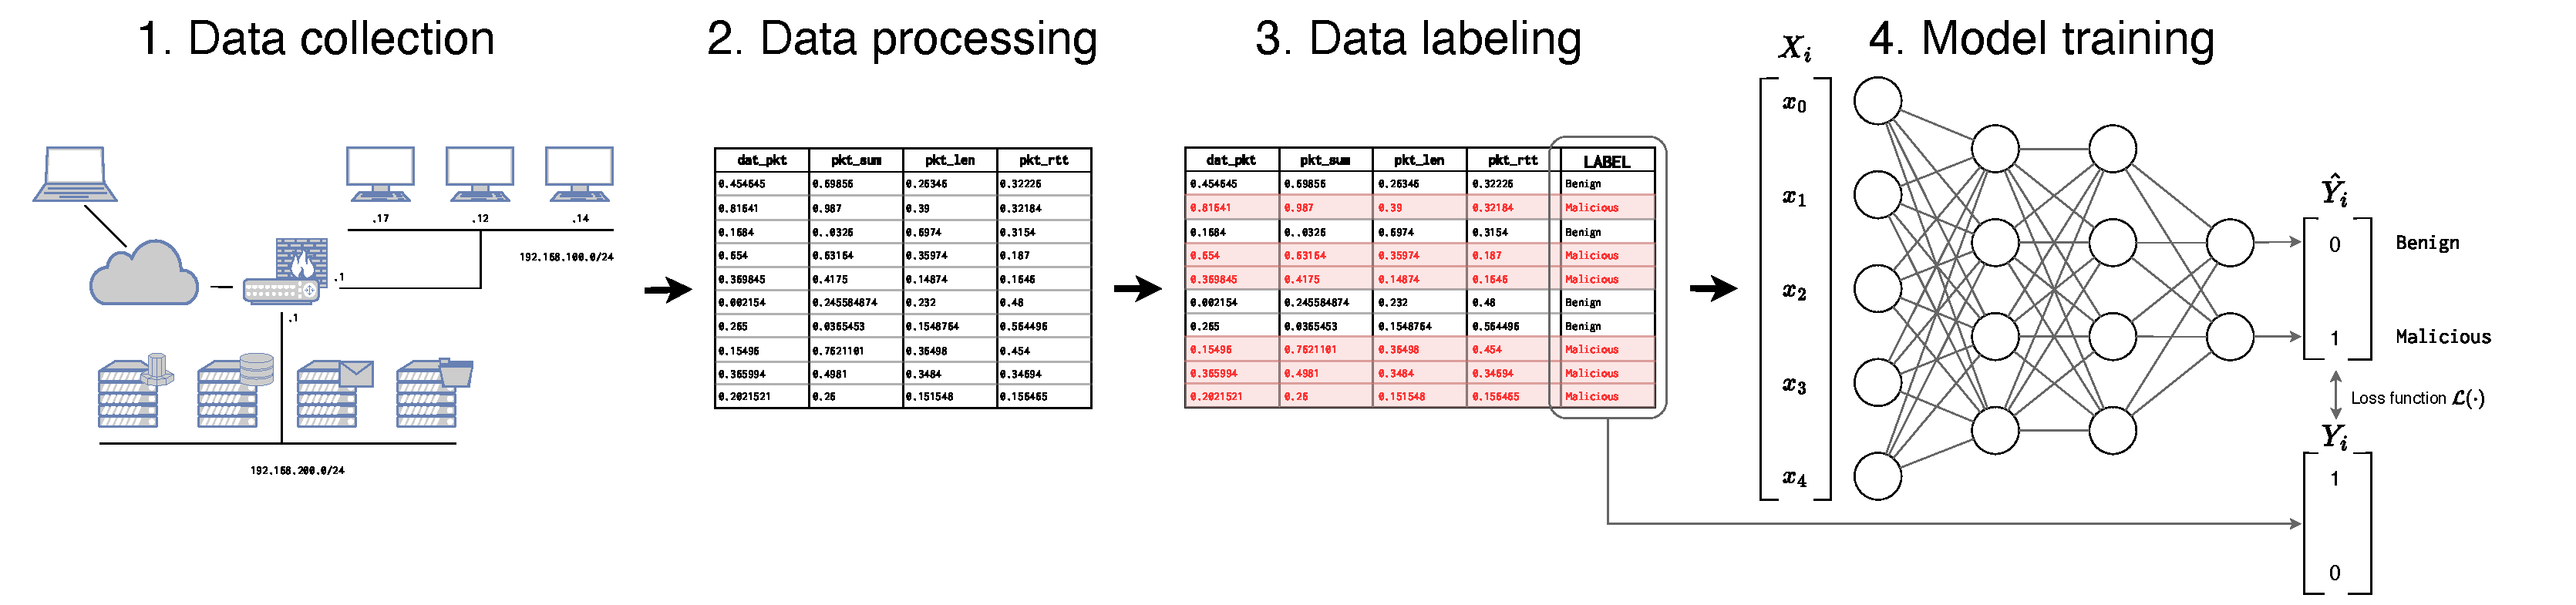
\includegraphics[width=.9\textwidth]{figures/intro/mlp-workflow.pdf}}
    \caption{Typical workflow for ML-based NIDSs.}
  \end{figure}
\end{frame}

\begin{frame}{Intrusion Detection}

  \begin{columns}
    \begin{column}{0.5\textwidth}
        \textbf{Challenges:}
        \begin{itemize}
          \item not enough labelled data;
          \item risk of local bias or skewed data distribution;
          \item inefficient against new attacks, especially \alert{supervised} approaches.
        \end{itemize}
    \end{column}

    \begin{column}{0.5\textwidth}
      \begin{figure}
        \centering
        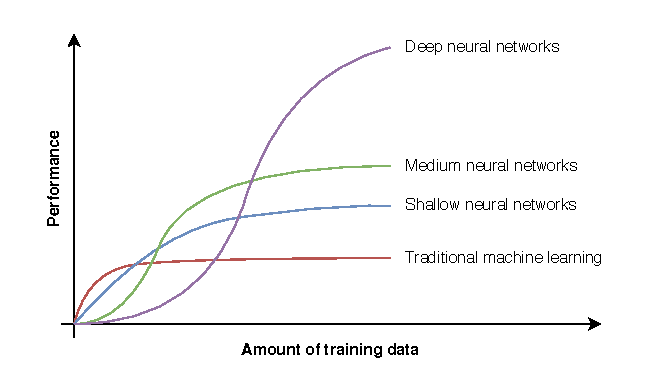
\includegraphics[width=\linewidth]{figures/intro/ml-perf}
      \end{figure}
    \end{column}
  \end{columns}
\end{frame}

\begin{frame}{Scaling Intrusion Detection}

  \textbf{Federated Learning (FL)}
  
  \begin{itemize}
    \item Novel-\emph{ish} distributed ML paradigm (Google, 2017)~\cite{mcmahan_Communicationefficientlearningdeep_2017}.
    \item Distributed clients can train a common model without sharing their training data.
    \item Privacy-preserving: high level of abstraction for the shared models preventing data leakage.
  \end{itemize}
\end{frame}

\begin{frame}{FL Fundamentals}
  \vspace{-1em}
  \begin{figure}
    \centering
    \only<1>{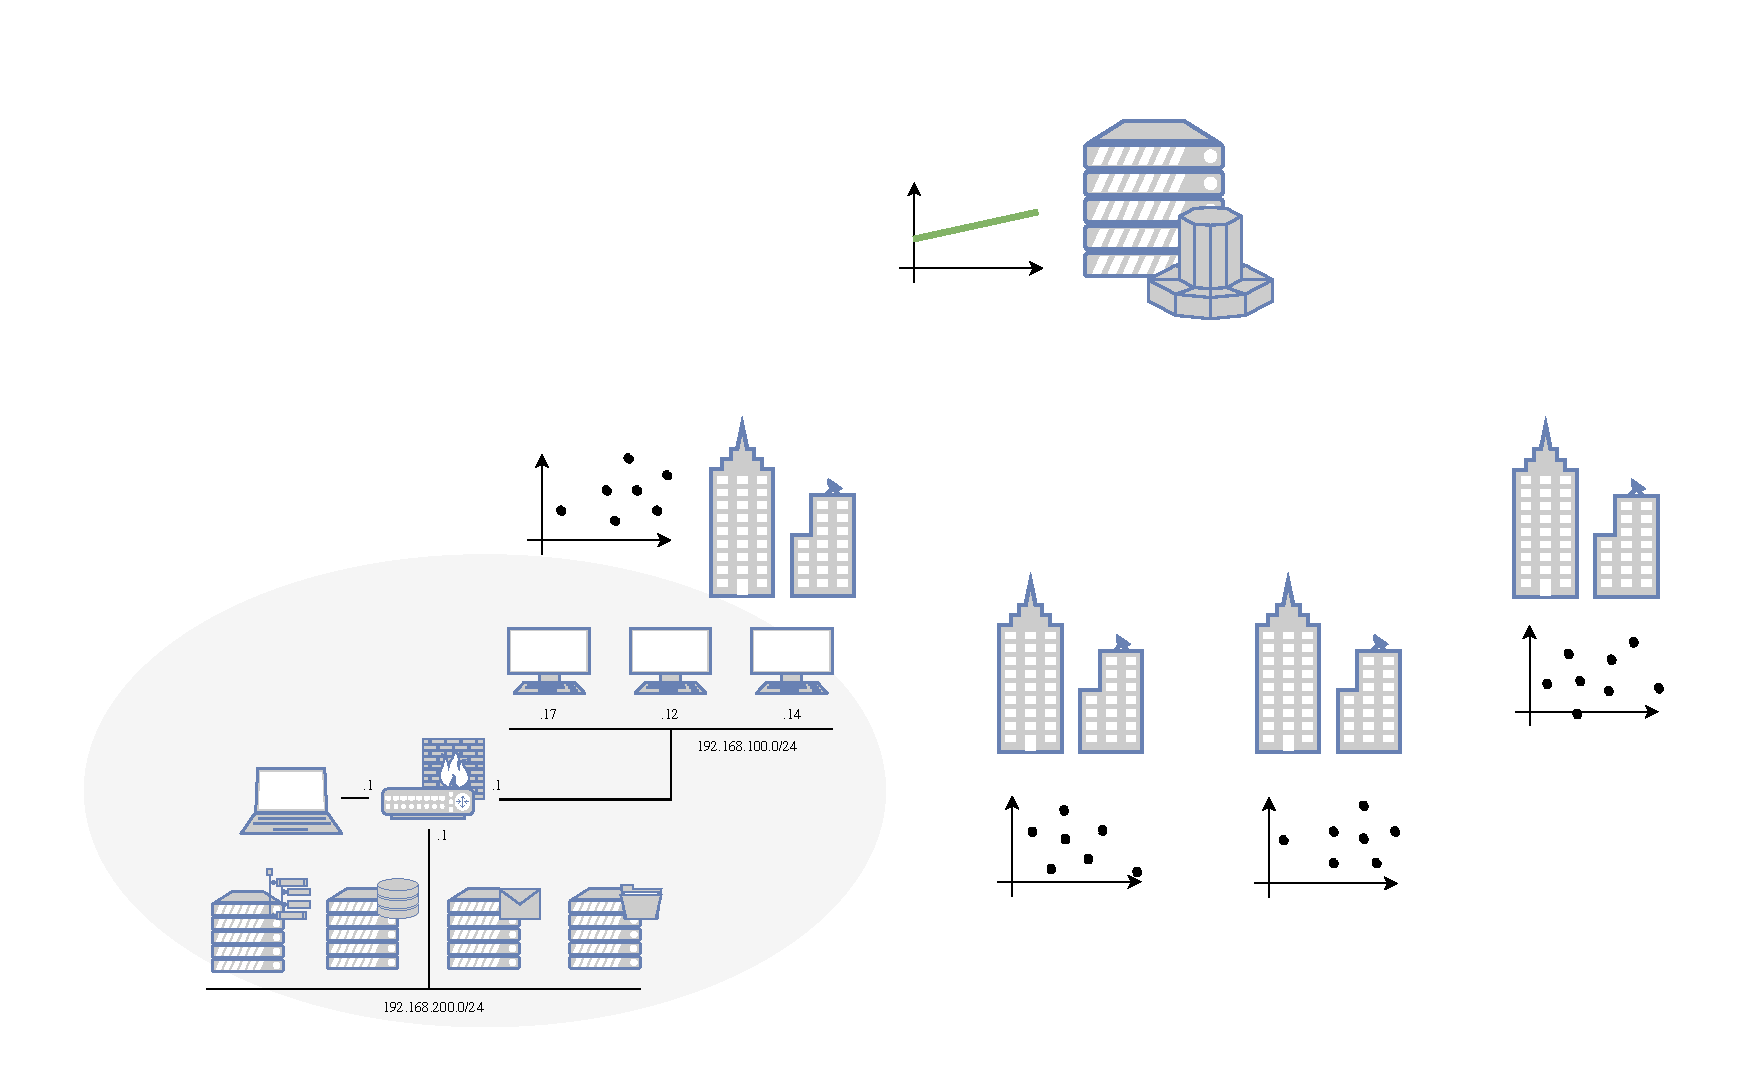
\includegraphics[width=.75\linewidth]{./figures/intro/fl/0.pdf}}%
    \only<2>{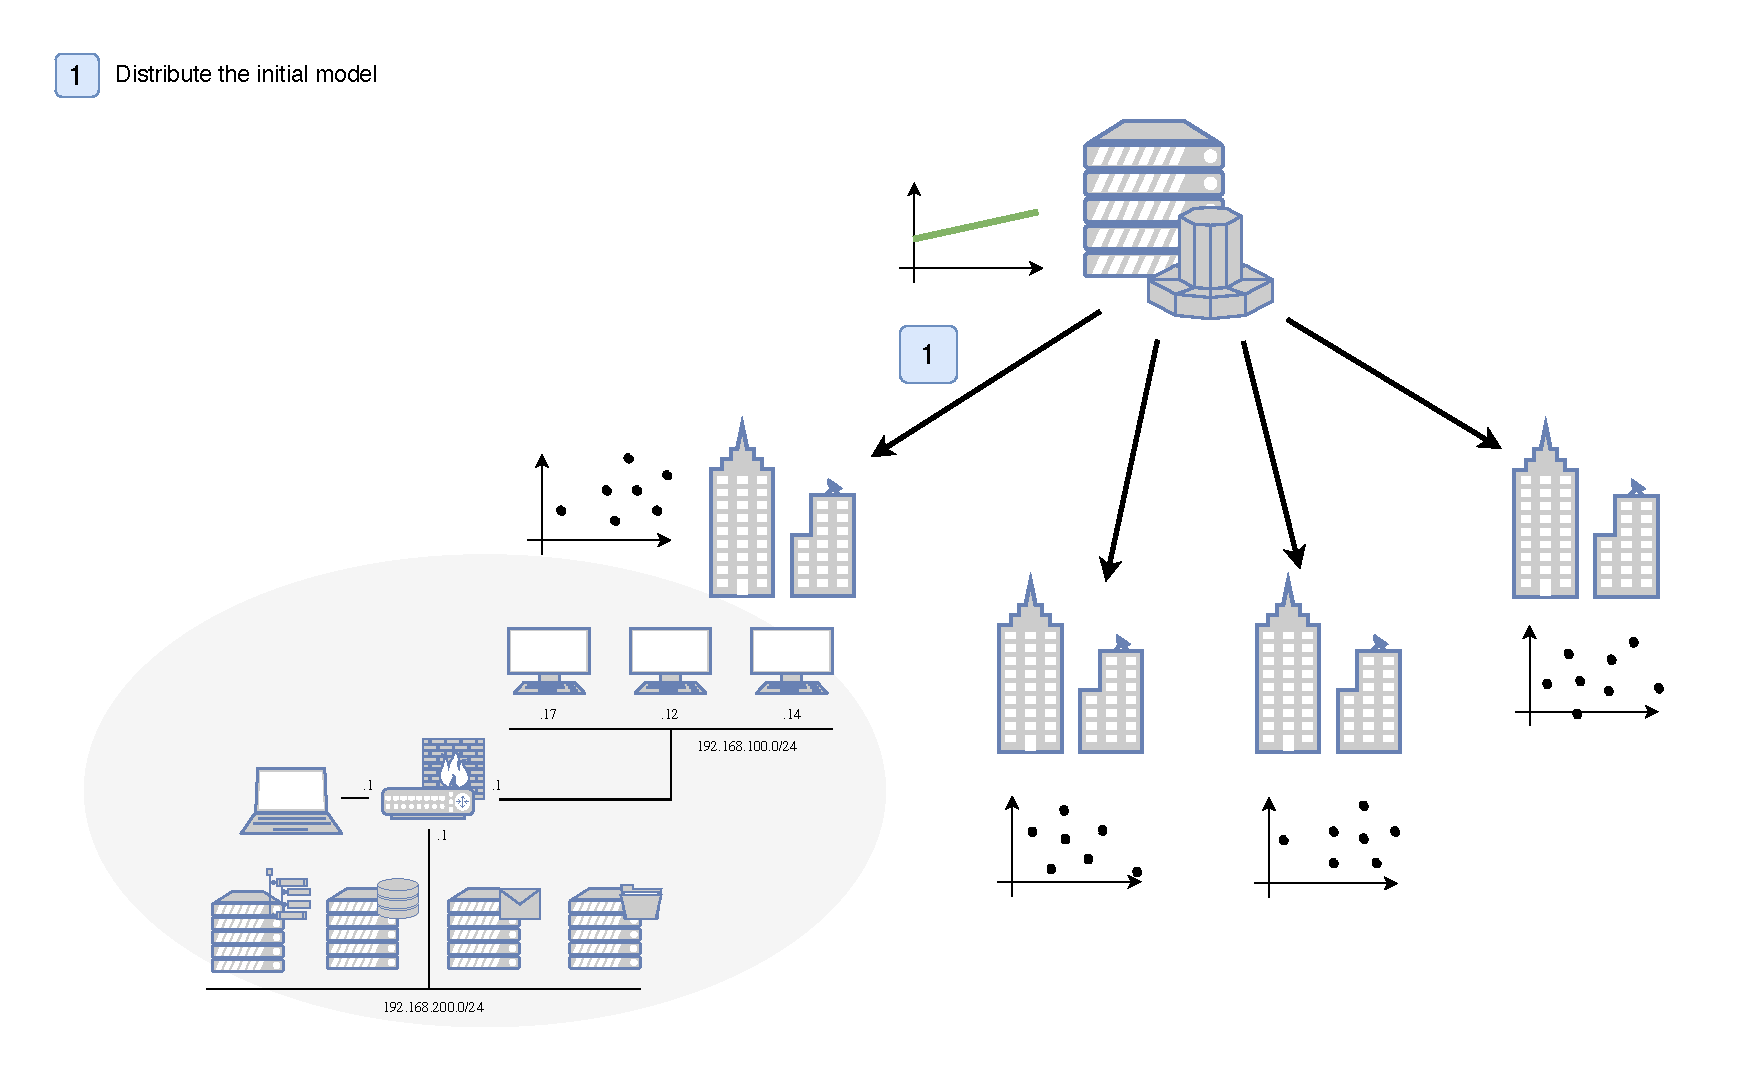
\includegraphics[width=.75\linewidth]{./figures/intro/fl/1.pdf}}%
    % Cannot use animations with MacOS Preview.
    % \only<3>{\animategraphics[width=.75\linewidth,loop,autoplay]{2}{./figures/intro/fl/2-}{1}{2}}%
    \only<3>{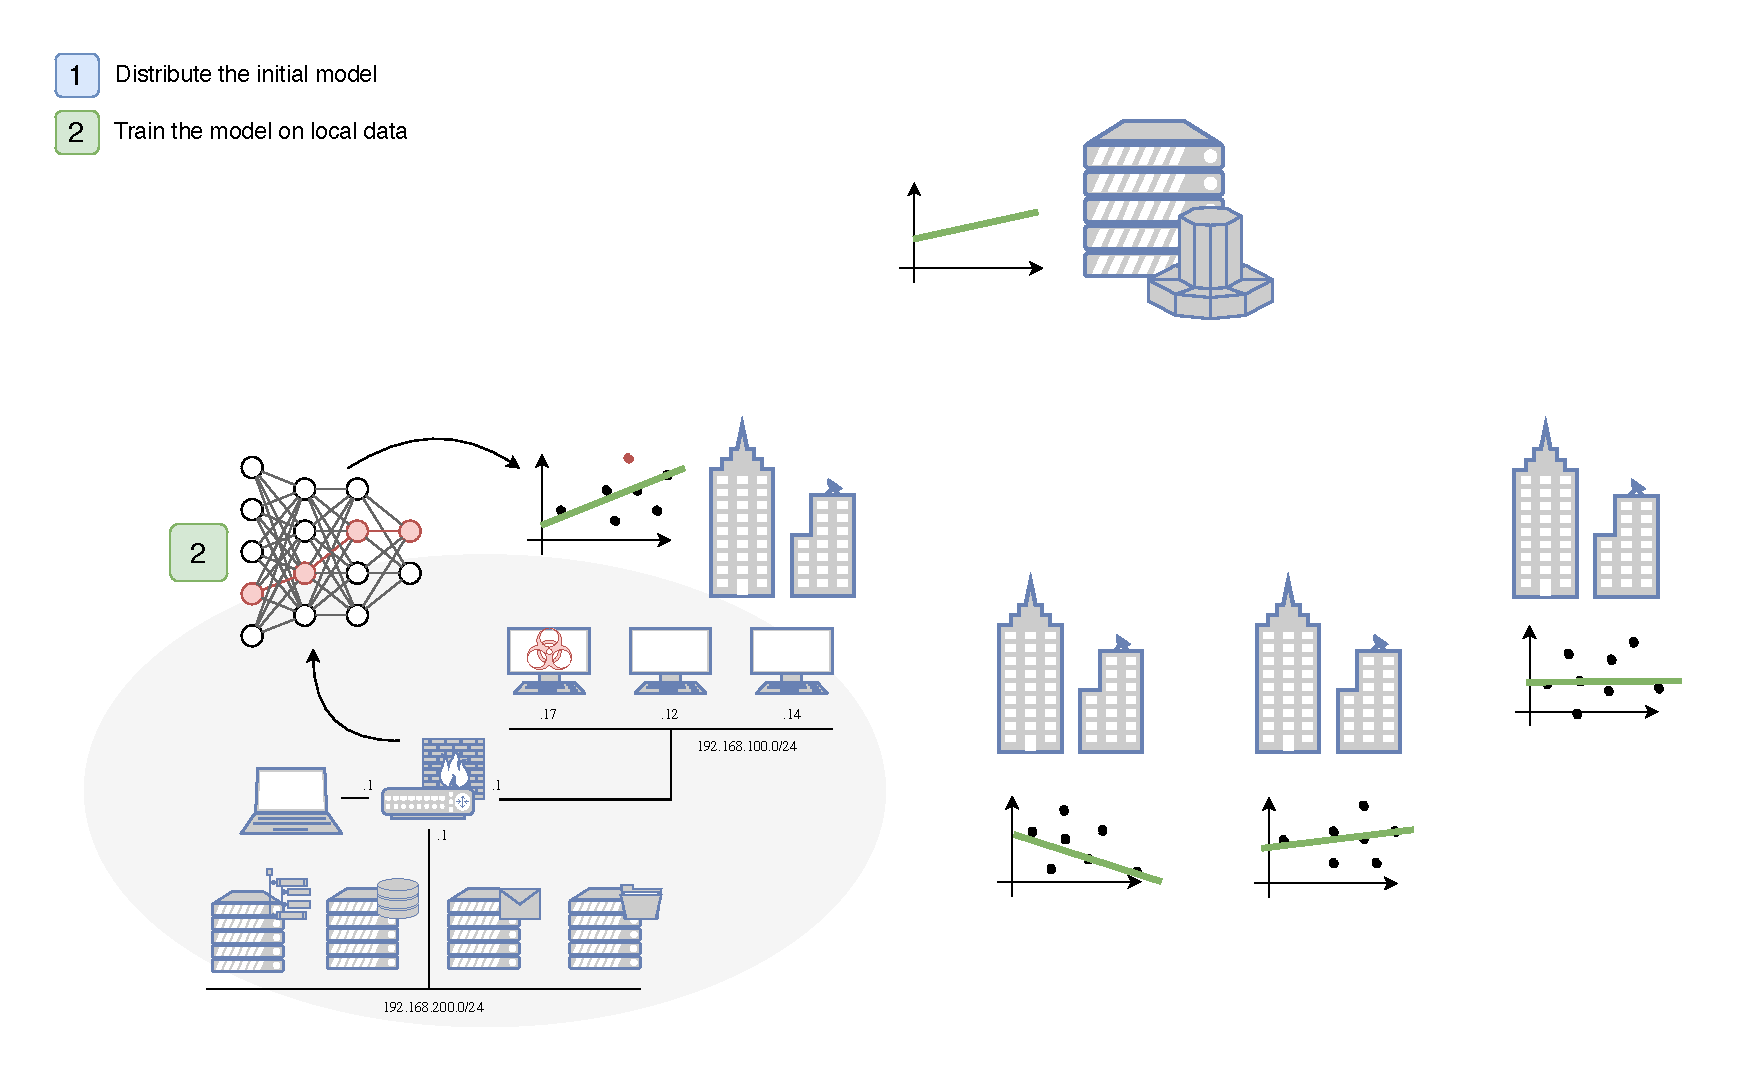
\includegraphics[width=.75\linewidth]{./figures/intro/fl/2-2.pdf}}%
    \only<4>{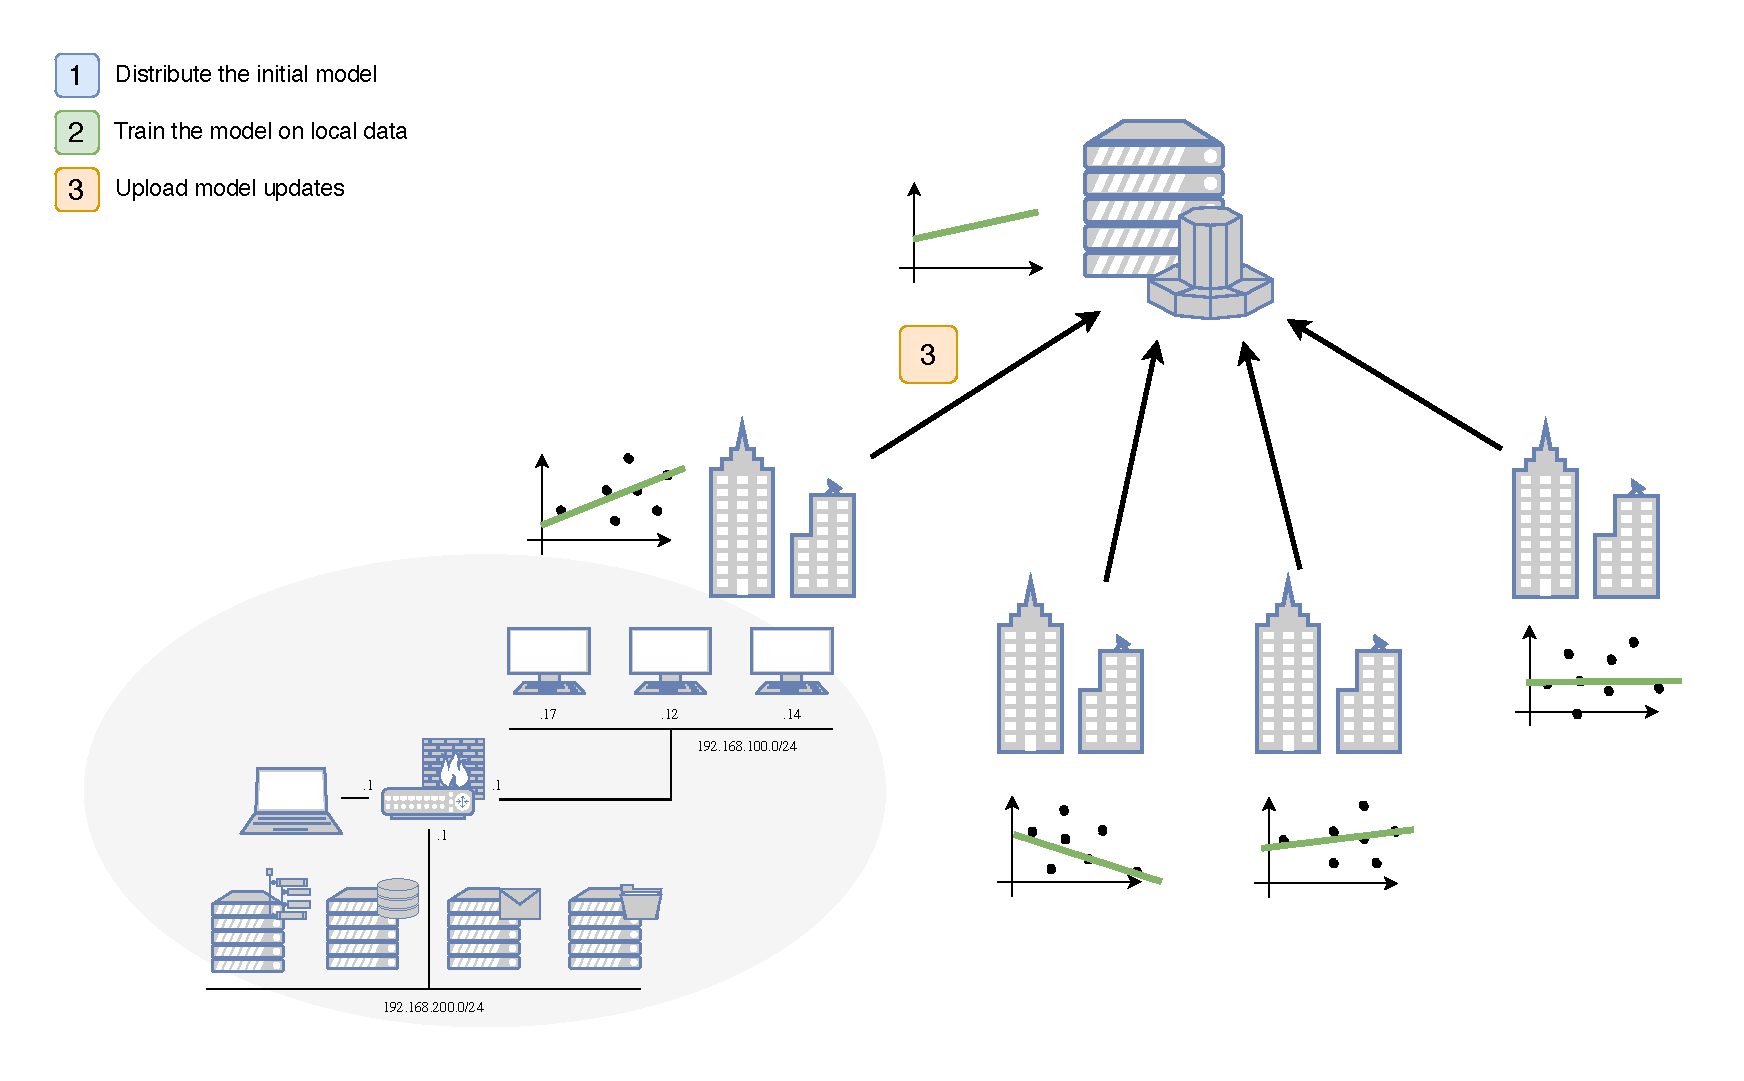
\includegraphics[width=.75\linewidth]{./figures/intro/fl/3.pdf}}%
    \only<5>{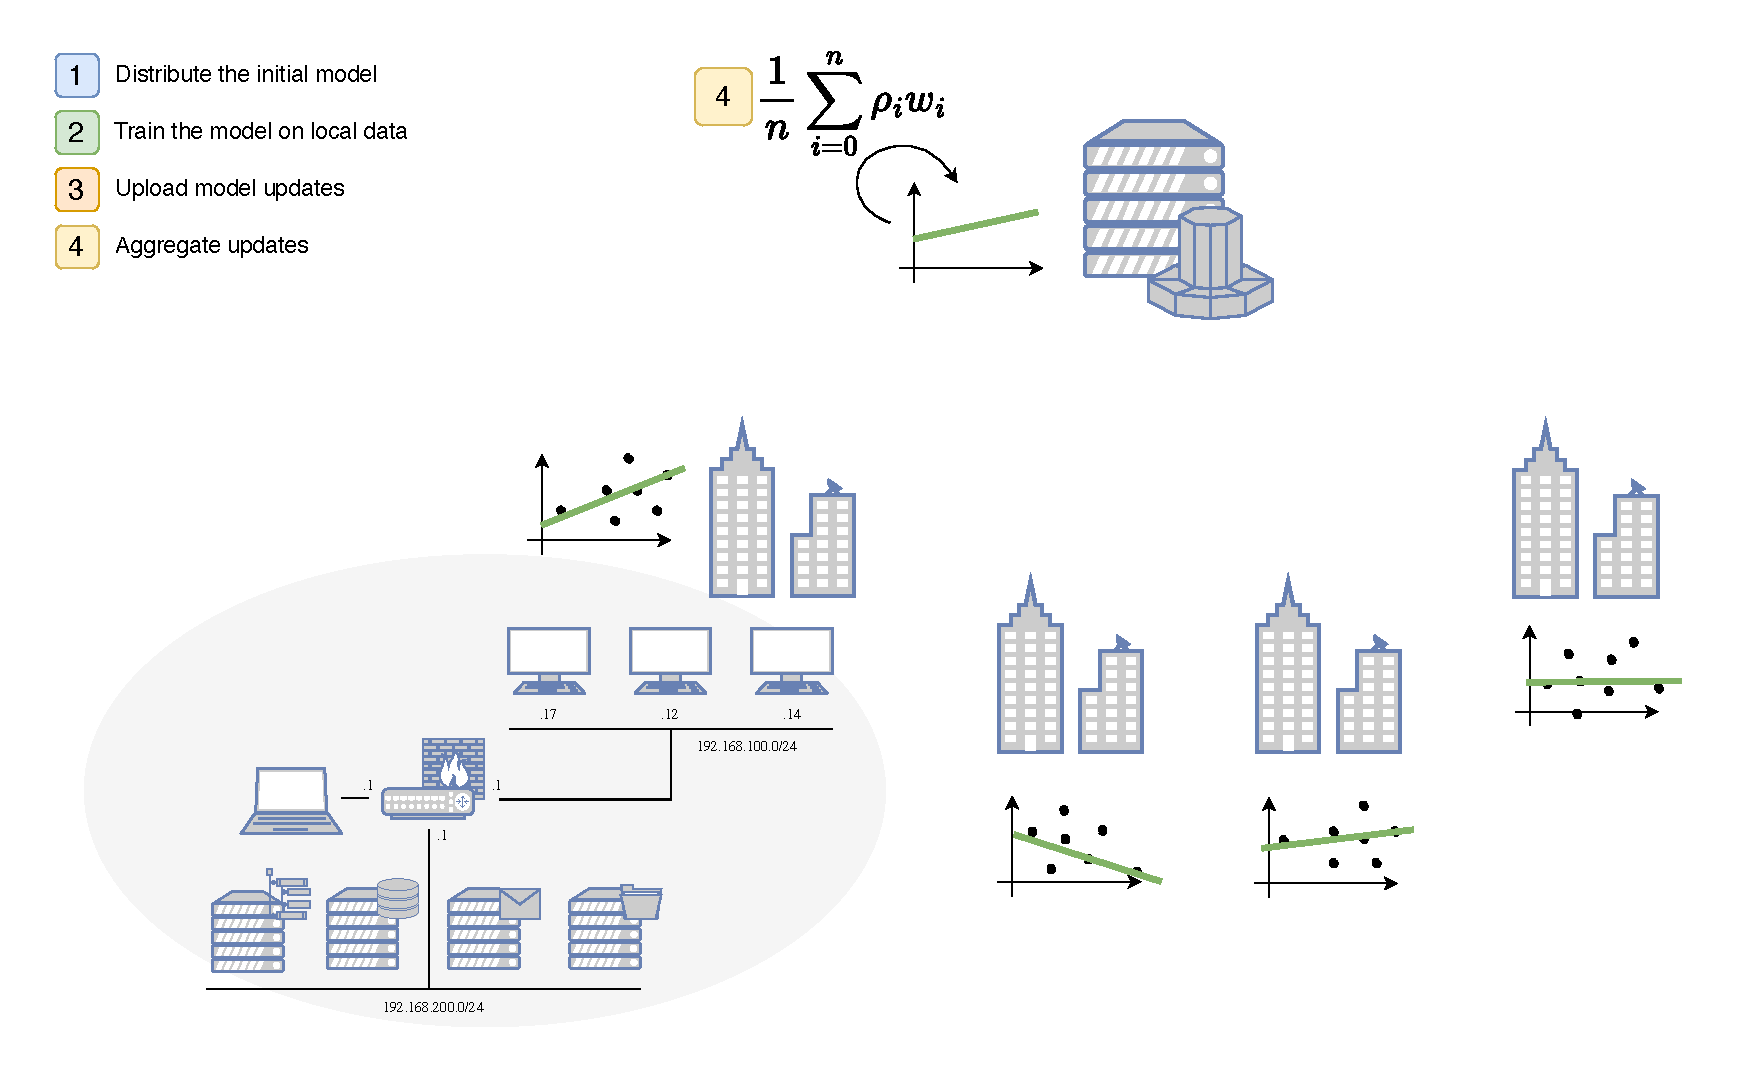
\includegraphics[width=.75\linewidth]{./figures/intro/fl/4.pdf}}%
    \only<6>{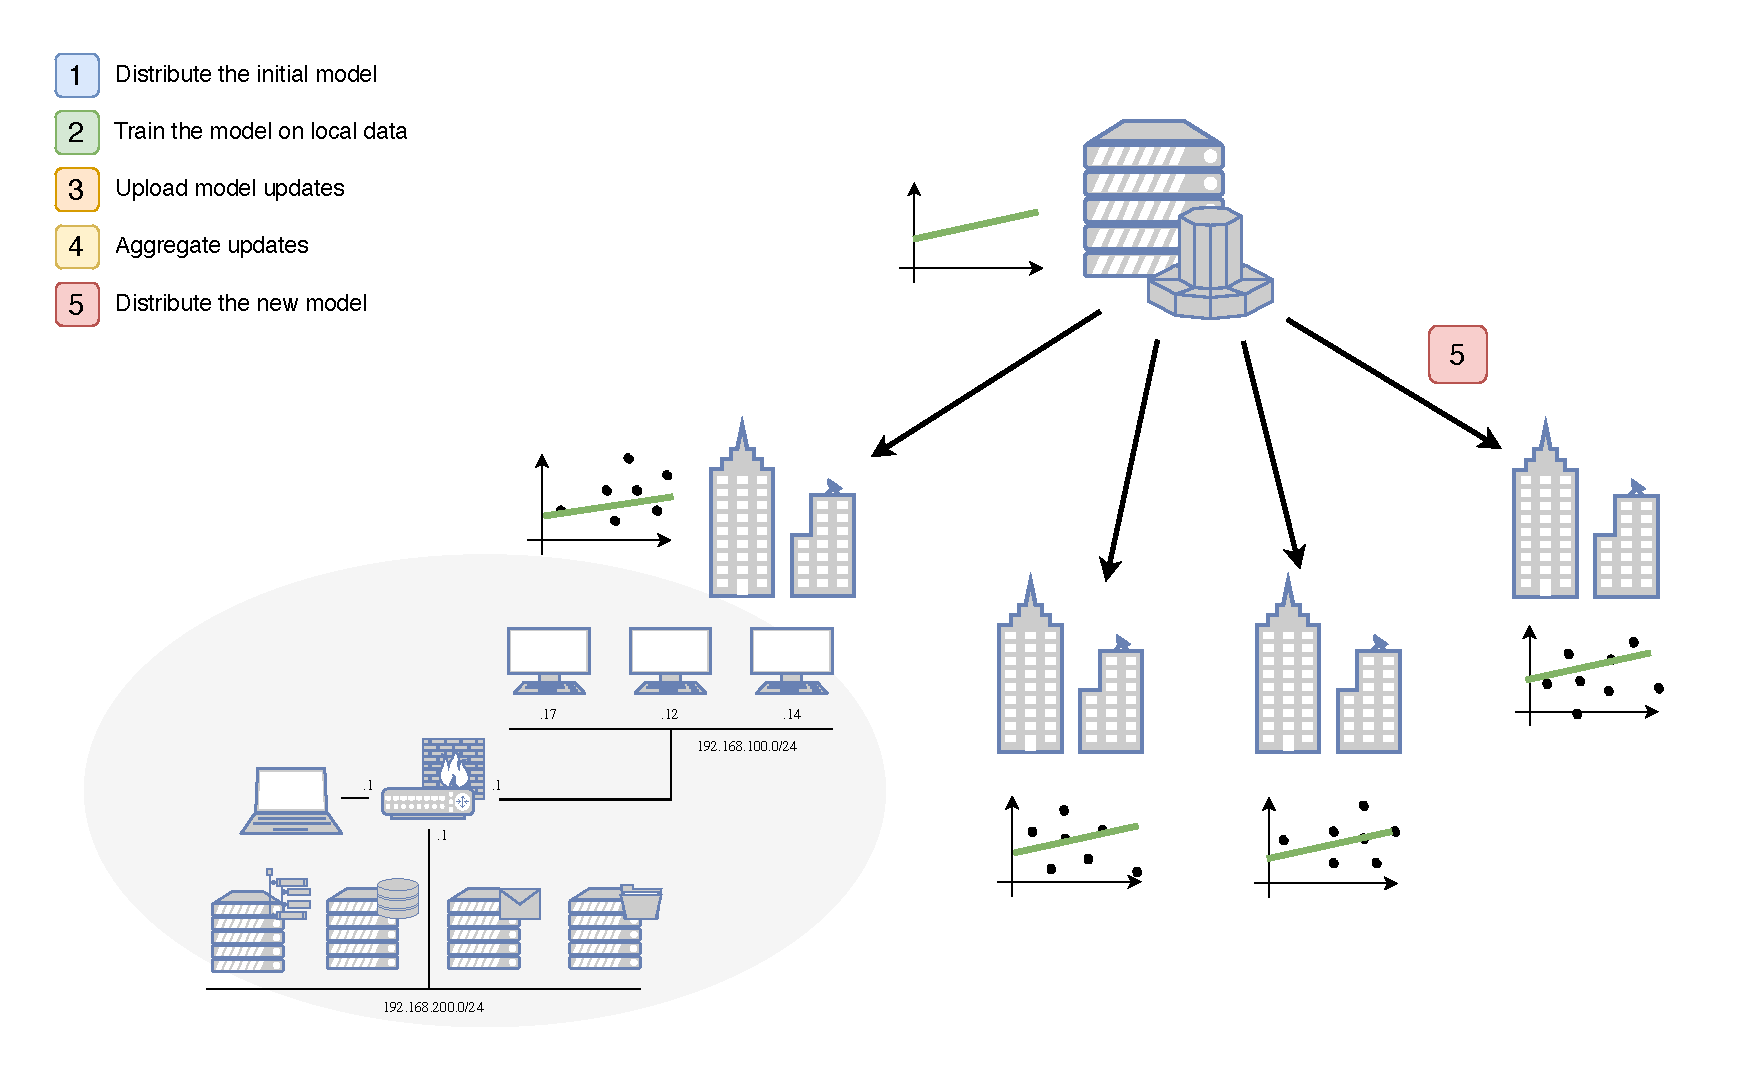
\includegraphics[width=.75\linewidth]{./figures/intro/fl/5.pdf}}%
    \only<7>{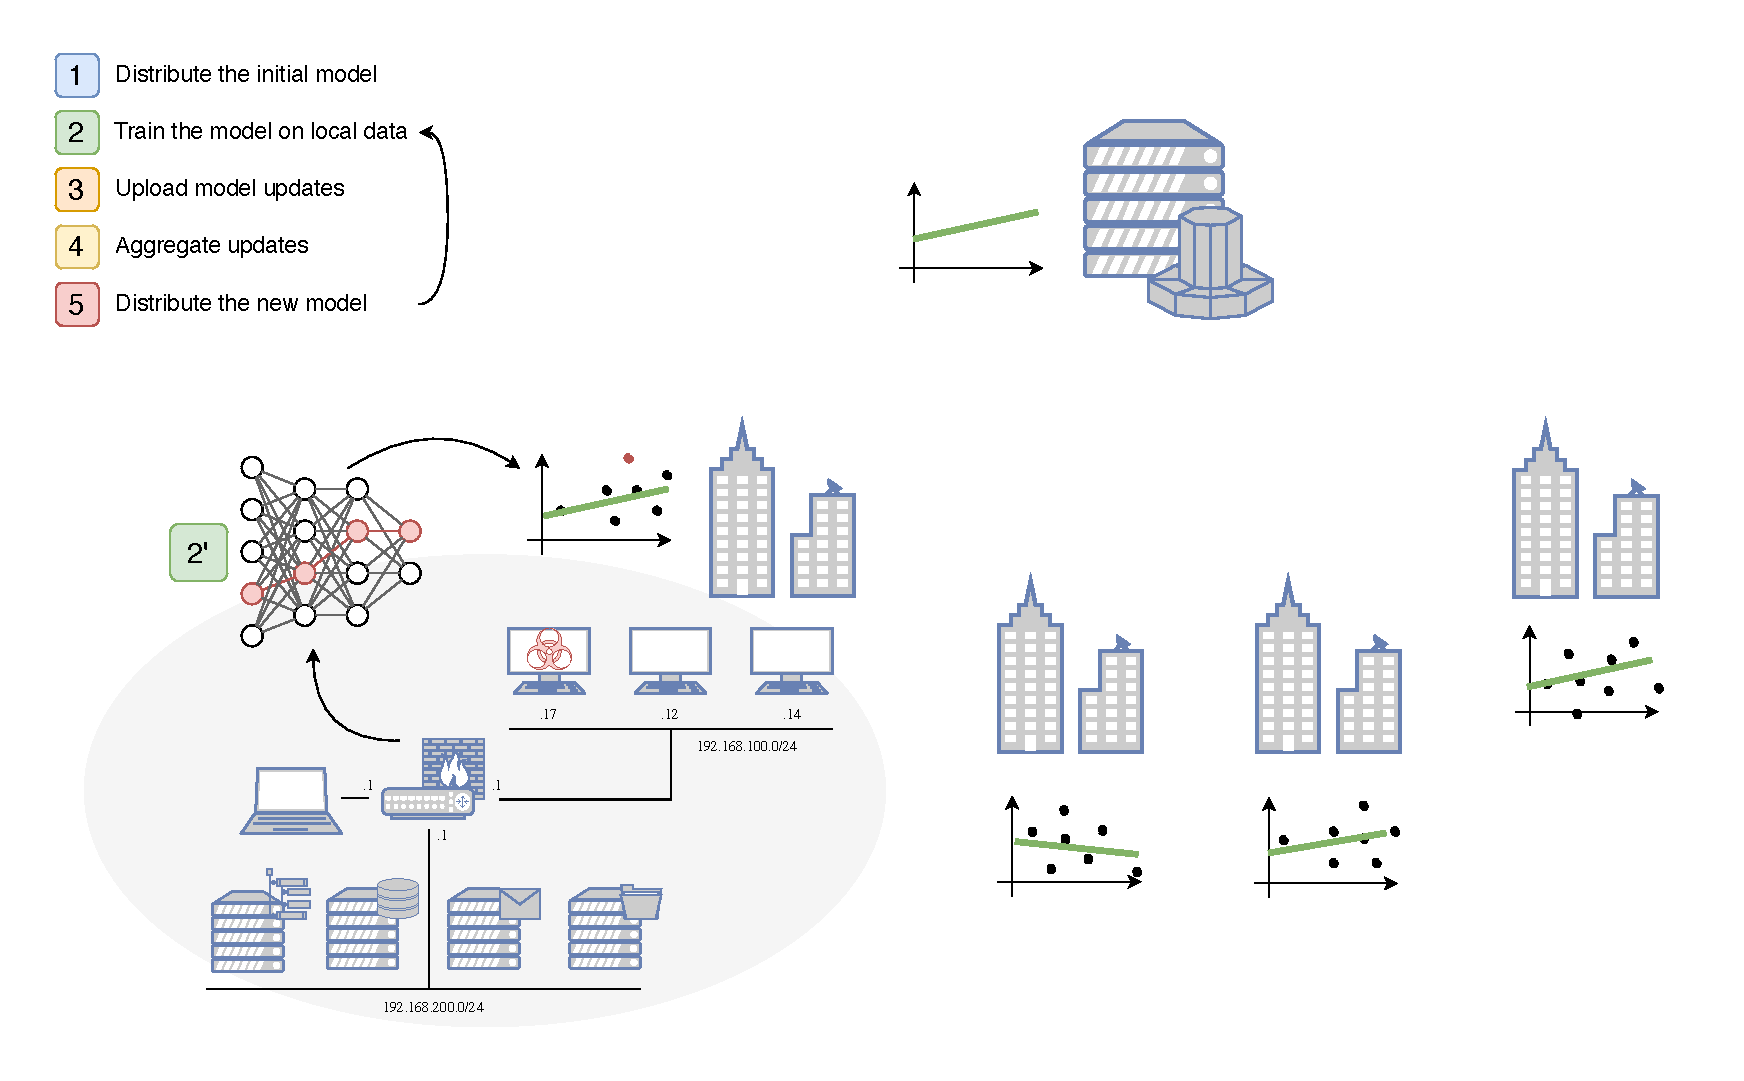
\includegraphics[width=.75\linewidth]{./figures/intro/fl/6.pdf}}%
    \caption{Typical FL workflow, applied to NIDSs.}
  \end{figure}
\end{frame}

\begin{frame}{FL for NIDSs}

  \textbf{Benefits}
  \begin{itemize}[<+->]
    \item Virtually extended dataset with Horizontal FL.
    \begin{itemize}[<1->]
      \item Better generalization.
      \item Reduced risk of overfitting or local bias.
    \end{itemize}
    

    \item Effectively share knowledge (\eg, on specific classes, instances) between participants
    \begin{itemize}[<1->]
      \item Share the knowledge about a new attack~\autocite{lavaur_icdcs_demo_2024};
      \item Improve the characterization of specific devices; \dots
    \end{itemize}

    \only<2>{\fcitefootnote{lavaur_icdcs_demo_2024}}

  \end{itemize}
\end{frame}


\end{document}
